%!TEX root = ../thesis.tex
%*******************************************************************************
%*********************************** First Chapter *****************************
%*******************************************************************************

\chapter{Trigger efficiency measurement}
\label{sec:Trigger}

In this chapter, the trigger configuration for the \ttbar production cross section measurement is described and the trigger efficiency is determined.
The trigger efficiency and its uncertainty are important parameters in measuring the \ttbar
production cross section. In previous analyses, the uncertainty on the trigger efficiency was one of the dominant uncertainties.
Similar to other efficiencies described in Chapter~\ref{sec:SimReco_Reco}, the trigger efficiency
is measured independently for both data and simulation, and the simulation is rescaled according to the efficiency measured in data.

The trigger selection used in this measurement 
is described in  Section~\ref{sec:TriggerSel}. 
The efficiency measurement itself is explained in Section~\ref{sec:TriggerMetMethod}, together with an alternative method. In order to estimate the precision of the trigger efficiency, another alternative method is applied,
as described in Section~\ref{sec:TriggerTPMethod}. The results from all three methods are compared in Section~\ref{sec:TriggerComp}.
The final set of scale factors between data and simulation used for the subsequent \ttbar cross section measurement is described in Section~\ref{sec:TrigSF}. 



%********************************** %First Section  **************************************
\section{Trigger selection} %Section - 1.1 
\label{sec:TriggerSel}

The trigger selection aims at reaching maximum efficiency, optimizing the amount of data available for the subsequent \ttbar production cross section measurement. 
Increasing the trigger efficiency also automatically reduces its statistical uncertainty, due to the statistical properties of the binomial distribution.
The trigger efficiency itself is measured with respect to the reconstructed and identified leptons (see Chapter~\ref{sec:SimReco_Reco} for details
on this reconstruction). The efficiencies of the trigger and offline selection factorize, \ie, they can be multiplied.

Several triggers, depending on the flavor of the
two leptons, are used in this analysis. Dilepton triggers typically have asymmetric \pt requirements for the two leptons, such that the leading lepton has a significantly higher \pt requirement than
the subleading lepton. Using single-lepton triggers for dilepton events has similar consequences. In general, particle properties reconstructed for the trigger are slightly different from the properties of particles used in the offline analysis. This
leads to an inefficiency of the trigger compared to the offline selection close to the trigger threshold.

In the case of the dilepton trigger this mainly affects the efficiency at the \pt threshold for the two leptons. One way to mitigate this is to
require a higher offline \pt for the leptons than is required by the trigger (see Section~\ref{sec:xsec_sel} for the offline selection).
Another way to reduce this inefficiency is to combine the dilepton trigger with other triggers which only depend on one lepton, mitigating any
inefficiency from the second lepton. Dilepton and single-lepton triggers are combined with a logical 'OR' in the trigger selection.

This combination increases the trigger efficiency by about ten percentage points compared to only using the dilepton trigger, as shown in Figure~\ref{fig:TriggerSel}.
The trigger selection is successfully optimized, since the trigger efficiency is close to $100\%$


\begin{figure}[htbp!]
  \begin{center}
    \resizebox{0.48 \textwidth}{!}{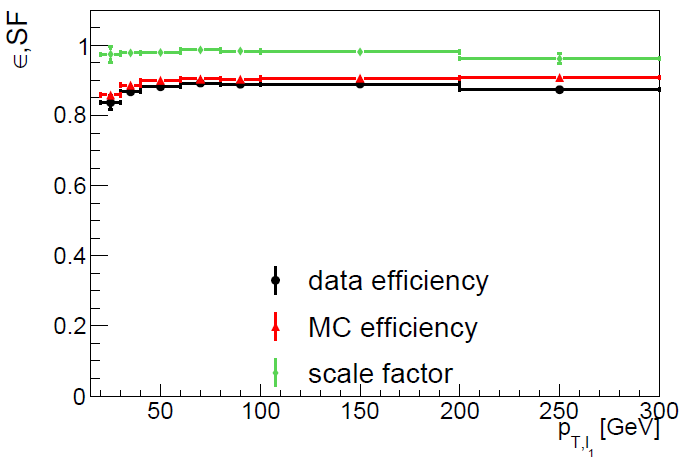
\includegraphics{Trigger/Figures/Trigger_pt_nosilep.png}}
    \resizebox{0.48 \textwidth}{!}{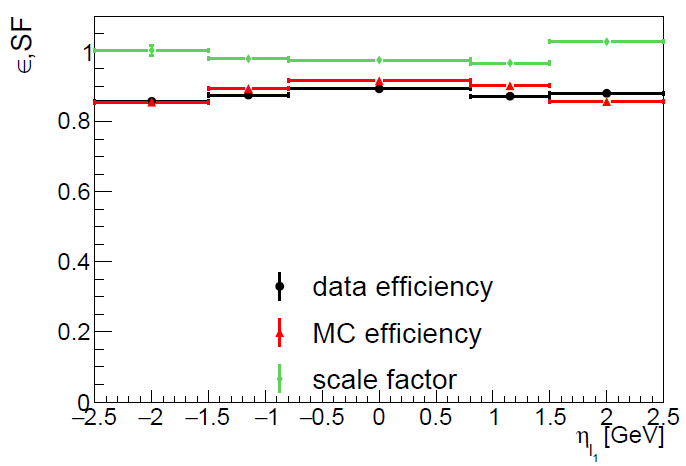
\includegraphics{Trigger/Figures/Trigger_eta_nosilep.png}}
    \resizebox{0.48 \textwidth}{!}{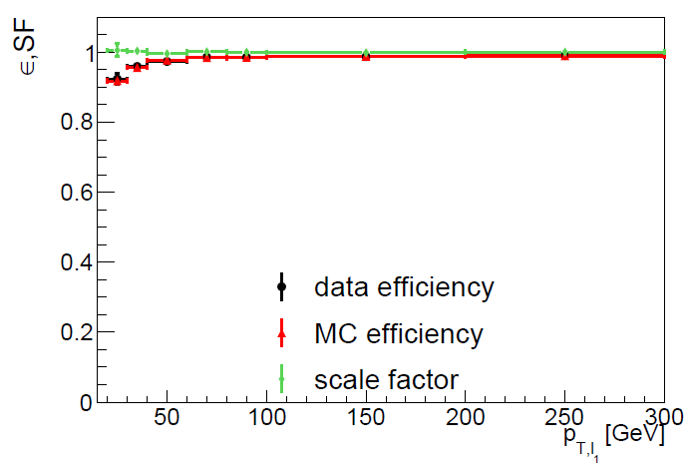
\includegraphics{Trigger/Figures/Trigger_pt.png}}
    \resizebox{0.48 \textwidth}{!}{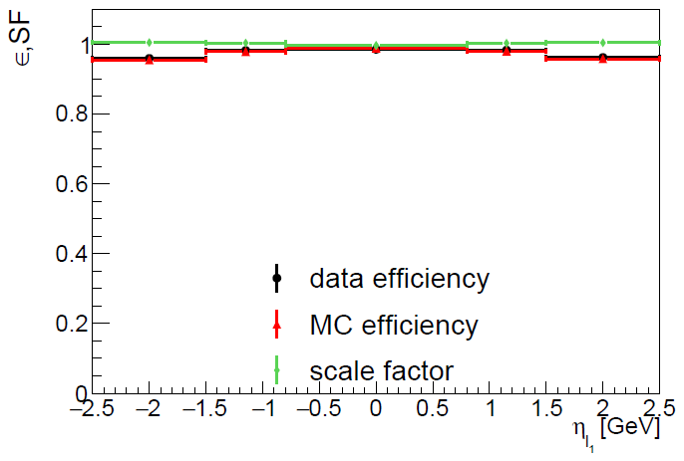
\includegraphics{Trigger/Figures/Trigger_eta.png}}
      \caption{Efficiencies of the trigger selection in the \emu channel for simulation and data and the corresponding scale factor. The upper row shows the efficiency when using dilepton triggers only, while the lower row shows
      the efficiency for a combination of dilepton and single-lepton triggers. The left column shows the efficiency as a function of the \pt of the leading lepton. The right column shows the efficiency as a function of  $\eta$ of the leading lepton. The data used for this comparison corresponds to an integrated luminosity of about $19\fbinv$.}  
       \label{fig:TriggerSel}
  \end{center}
\end{figure}


Because of changing conditions during data taking, certain trigger configurations are only available for certain periods of data taking. The triggers chosen here give the most relaxed kinematic requirements possible.
This results in the trigger selection depending on the data taking period, as shown in Table~\ref{tab:triggerSel} for each of the three dilepton channels.

Events triggered with certain classes of triggers (such as single-muon or single-electron triggers) are written so separate data sets, leading
to a possible overlap when combining these data sets.
Double counting of events is prevented by explicitly requiring triggers in their respective data set, but vetoing them in the other data sets.

\begin{table}[hbt]
    \centering
    \caption{The trigger selection applied on data. It differs between the different run periods because of changing trigger configurations.}
    \label{tab:triggerSel}
     \begin{tabular}
            {c|c|l}
            Channel & Run & Trigger \\
            \hline
             \mumu & B-G & Mu17\_TrkIsoVVL\_Mu8\_TrkIsoVVL \\
              & B-G & Mu17\_TrkIsoVVL\_TkMu8\_TrkIsoVVL \\
              & H & Mu17\_TrkIsoVVL\_Mu8\_TrkIsoVVL\_DZ \\
              & H & Mu17\_TrkIsoVVL\_TkMu8\_TrkIsoVVL\_DZ \\
              & B-H & IsoMu24 \\
              & B-H & IsoTkMu24 \\
            \hline
             \ee &  B-H & Ele23\_Ele12\_CaloIdL\_TrackIdL\_IsoVL\_DZ \\
              &  B-H & Ele27\_WPTight\_Gsf \\
            \hline
             \empm & B-G & Mu23\_TrkIsoVVL\_Ele12\_CaloIdL\_TrackIdL\_IsoVL \\
              & B-G & Mu8\_TrkIsoVVL\_Ele23\_CaloIdL\_TrackIdL\_IsoVL \\
              & H & Mu23\_TrkIsoVVL\_Ele12\_CaloIdL\_TrackIdL\_IsoVL\_DZ \\
              & H & Mu8\_TrkIsoVVL\_Ele23\_CaloIdL\_TrackIdL\_IsoVL\_DZ \\
              & B-H & Ele27\_WPTight\_Gsf \\
              & B-H & IsoMu24 \\
              & B-H & IsoTkMu24 \\
    \end{tabular}
\end{table}







%********************************** %Second Section  *************************************
\section{Methods using independent triggers} %Section - 1.2
\label{sec:TriggerMetMethod}

In this analysis, the trigger efficiency is mainly measured using a data set taken with triggers that are independent from the lepton triggers.
In general, this allows to measure the trigger efficiency without bias in data and simulation independently. 
It is important that these independent triggers are as uncorrelated with the lepton triggers as possible.  
In this Section two methods, with two different sets of independent triggers, are described.

Here, triggers based on the missing transverse energy (\ETm) are used. They are especially useful for a \ttbar analysis, 
as dileptonic \ttbar events are expected to produce \ETm due to the two neutrinos. Choosing triggers based on \ETm allows measuring the trigger efficiency for data
in an event sample that contains \ttbar events. The efficiency in simulation can be measured in a sample of \ttbar events.
The correlation between the \ETm and dilepton triggers is studied in simulation and found to be minimal.

As an alternative, the efficiency of the single-lepton triggers can be measured in an \emu data set.
This method is used to determine the systematic uncertainty on the trigger efficiency measurement by comparing these efficiencies to single lepton trigger efficiencies determined with \ETm triggers.

The trigger efficiency is measured by dividing the amount of events that pass both the offline selection and the dilepton trigger by the number of events that only pass the offline selection.
All events have to pass the \ETm triggers in order to guarantee an unbiased sample. The efficiency is defined as follows: 

\begin{equation}
\varepsilon_{trig} = \frac{N(\mathrm{Offline\; selection + \ETm \; trigger + dilepton\; trigger})}{N(\mathrm{offline\; selection + \ETm \; trigger})},
\label{eq:TriggerEff}
\end{equation}

where $N$ denotes the number of events that fulfill the given requirements.

The efficiency is measured per event, so the resulting scale factors, to correct simulation to data, are applied per event as well.
This is especially useful if a combination of multiple triggers is used in the trigger selection.

The statistical uncertainty is calculated assuming a binomial distribution using the Clopper-Pearson method~\cite{10.2307/2331986,2010NIMPA.612..388C}. It offers at least nominal coverage 
of the given confidence level and a conservative option to estimate the uncertainty. 

Results for efficiencies and scale factors for the \ee, \mumu, and \emu channel are shown in Figures~\ref{fig:MET_ee},~\ref{fig:MET_mumu}, and~\ref{fig:MET_emu}, respectively.

\begin{figure}[htbp!]
  \begin{center}
    \resizebox{0.48 \textwidth}{!}{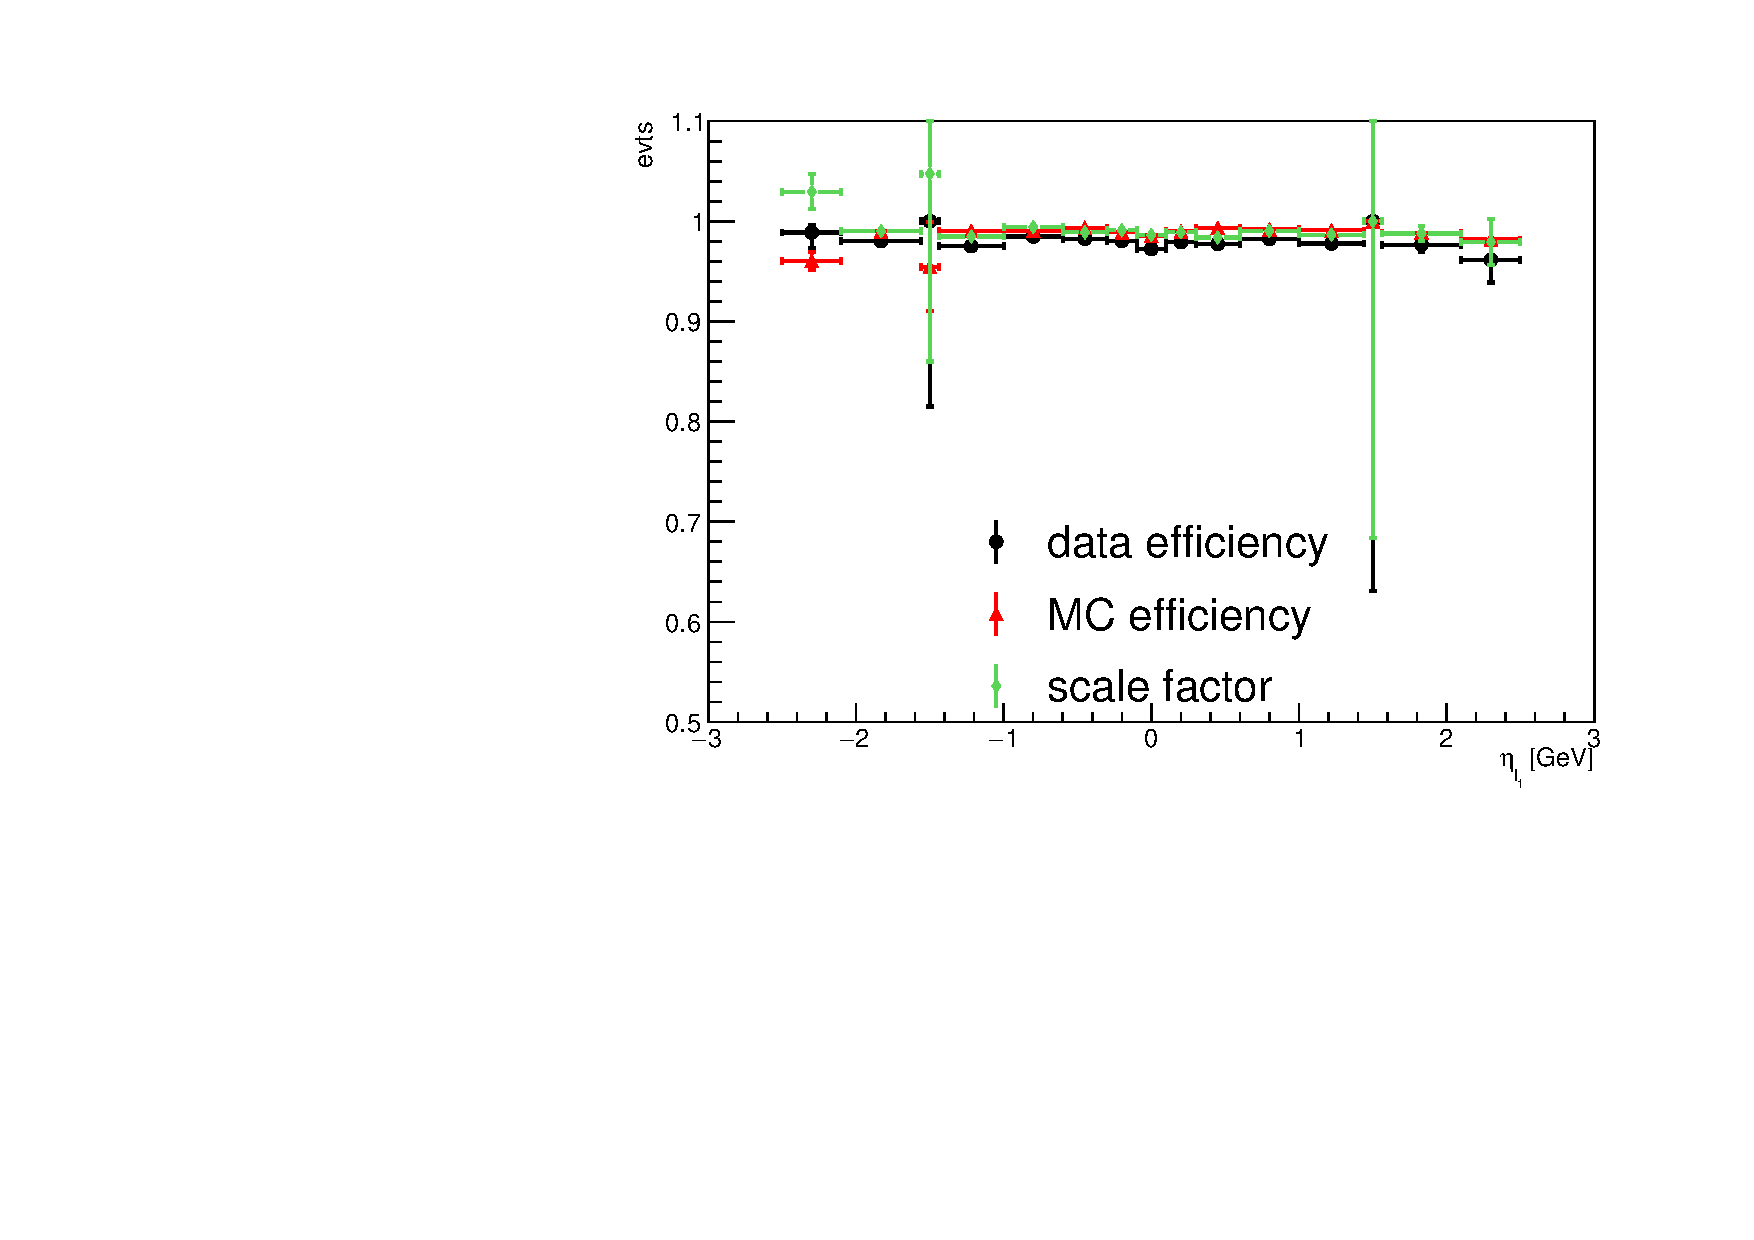
\includegraphics{Trigger/Figures/MET/ee/leading_eta}}
    \resizebox{0.48 \textwidth}{!}{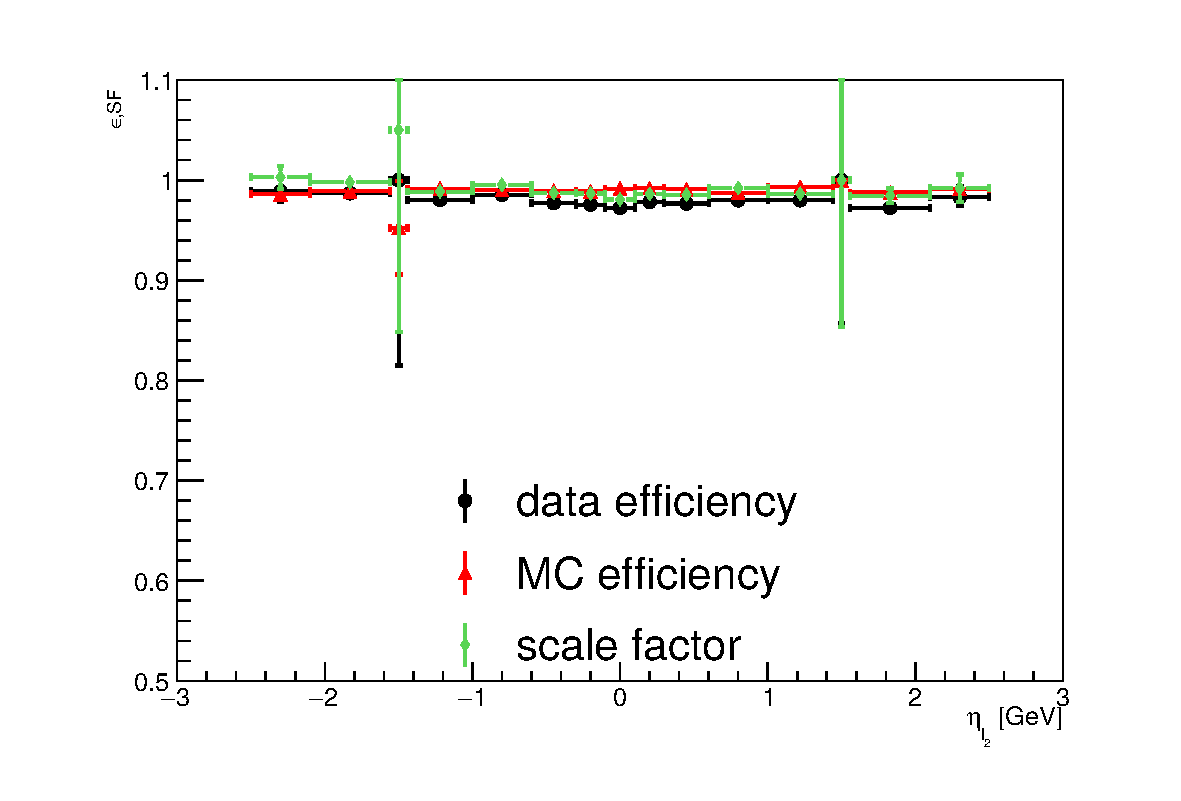
\includegraphics{Trigger/Figures/MET/ee/seleading_eta}}
    \resizebox{0.48 \textwidth}{!}{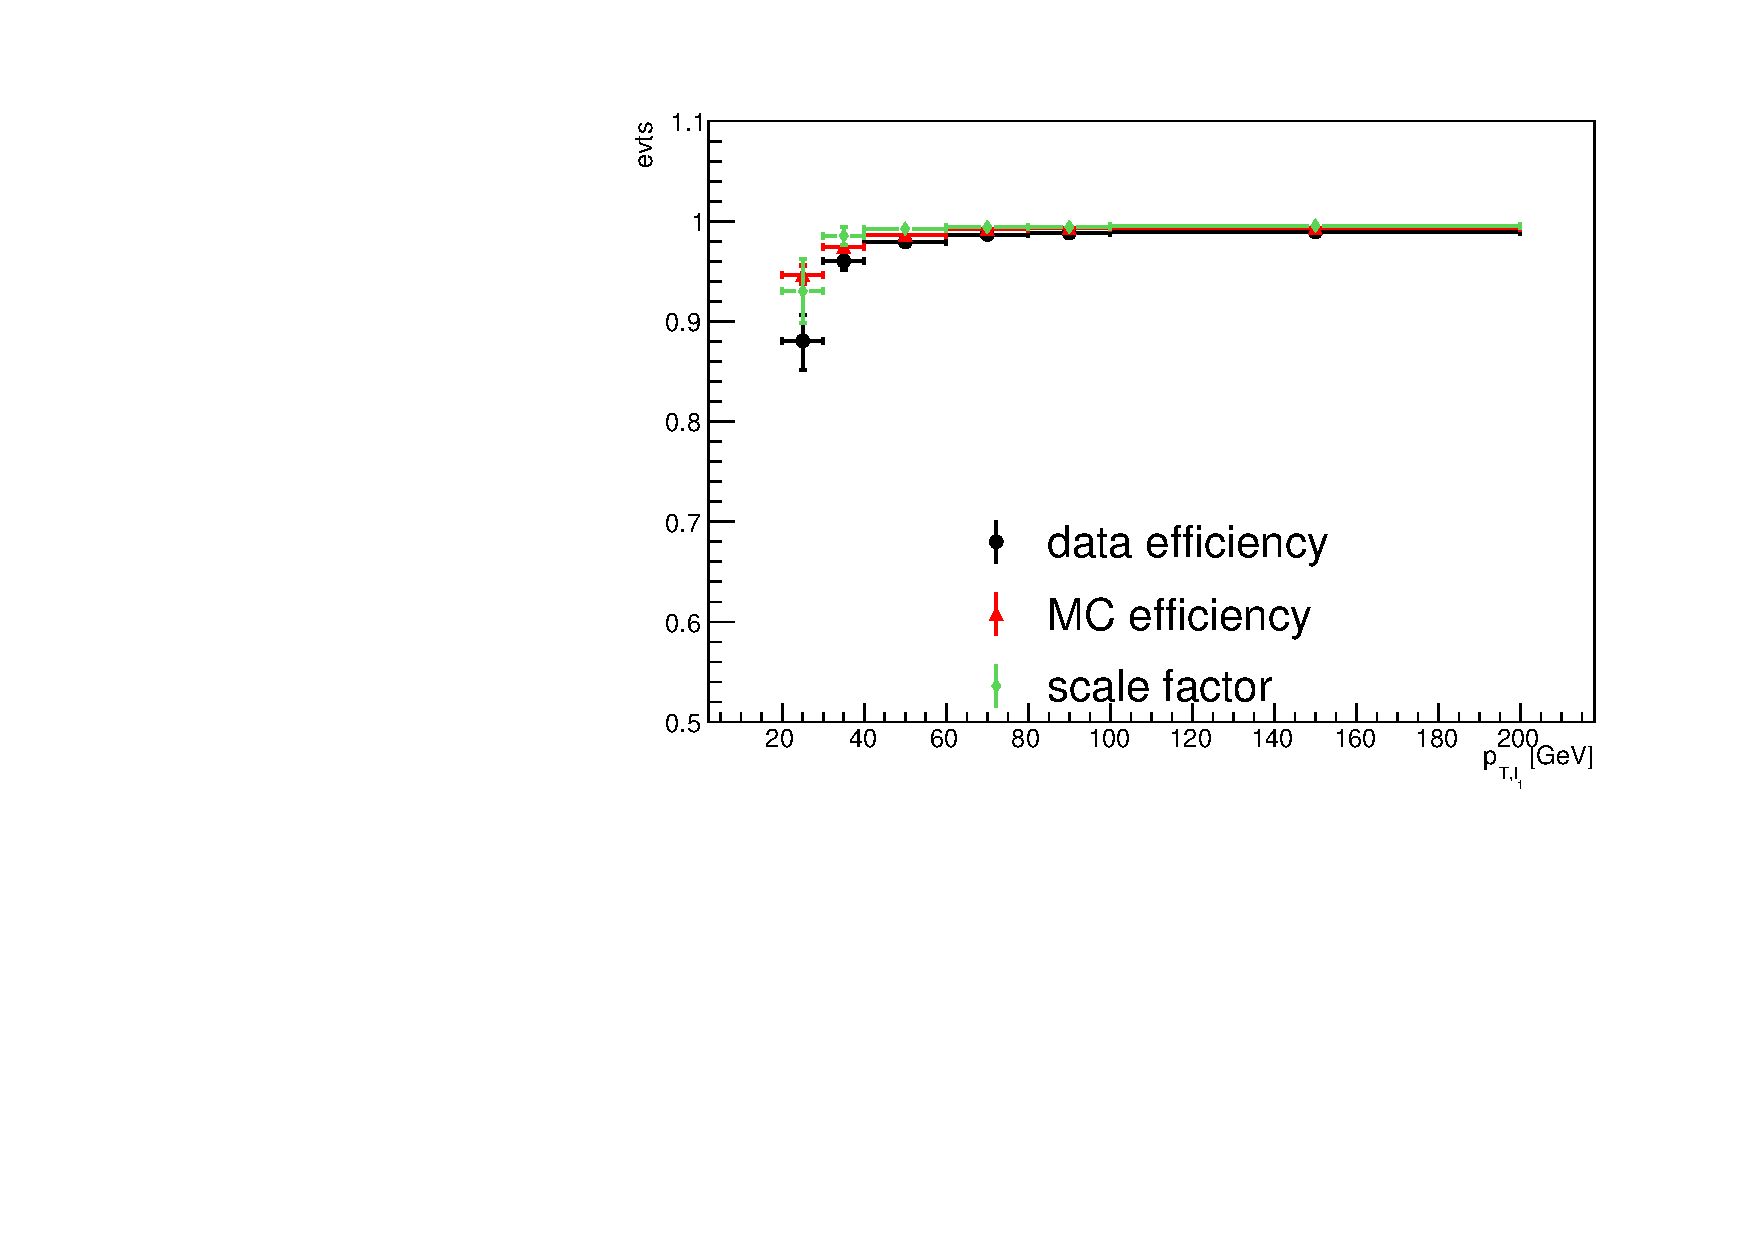
\includegraphics{Trigger/Figures/MET/ee/leading_pt}}
    \resizebox{0.48 \textwidth}{!}{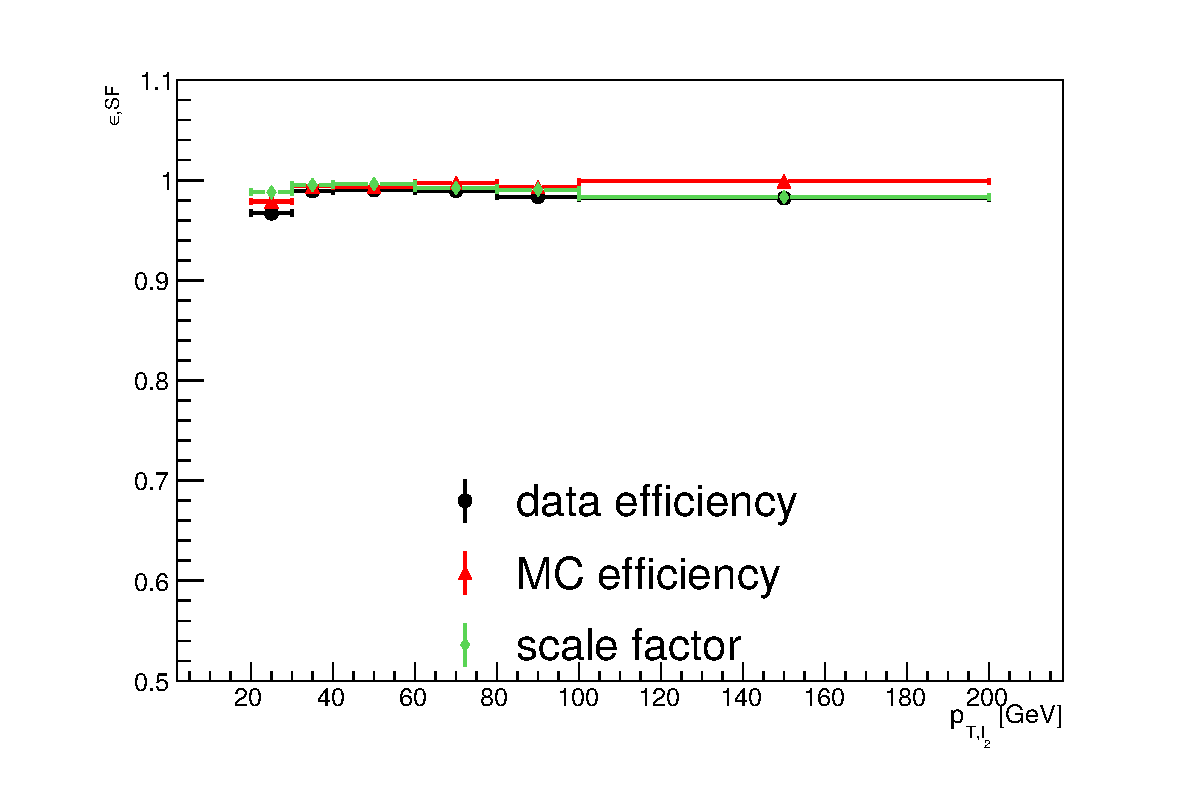
\includegraphics{Trigger/Figures/MET/ee/seleading_pt}}
    \resizebox{0.48 \textwidth}{!}{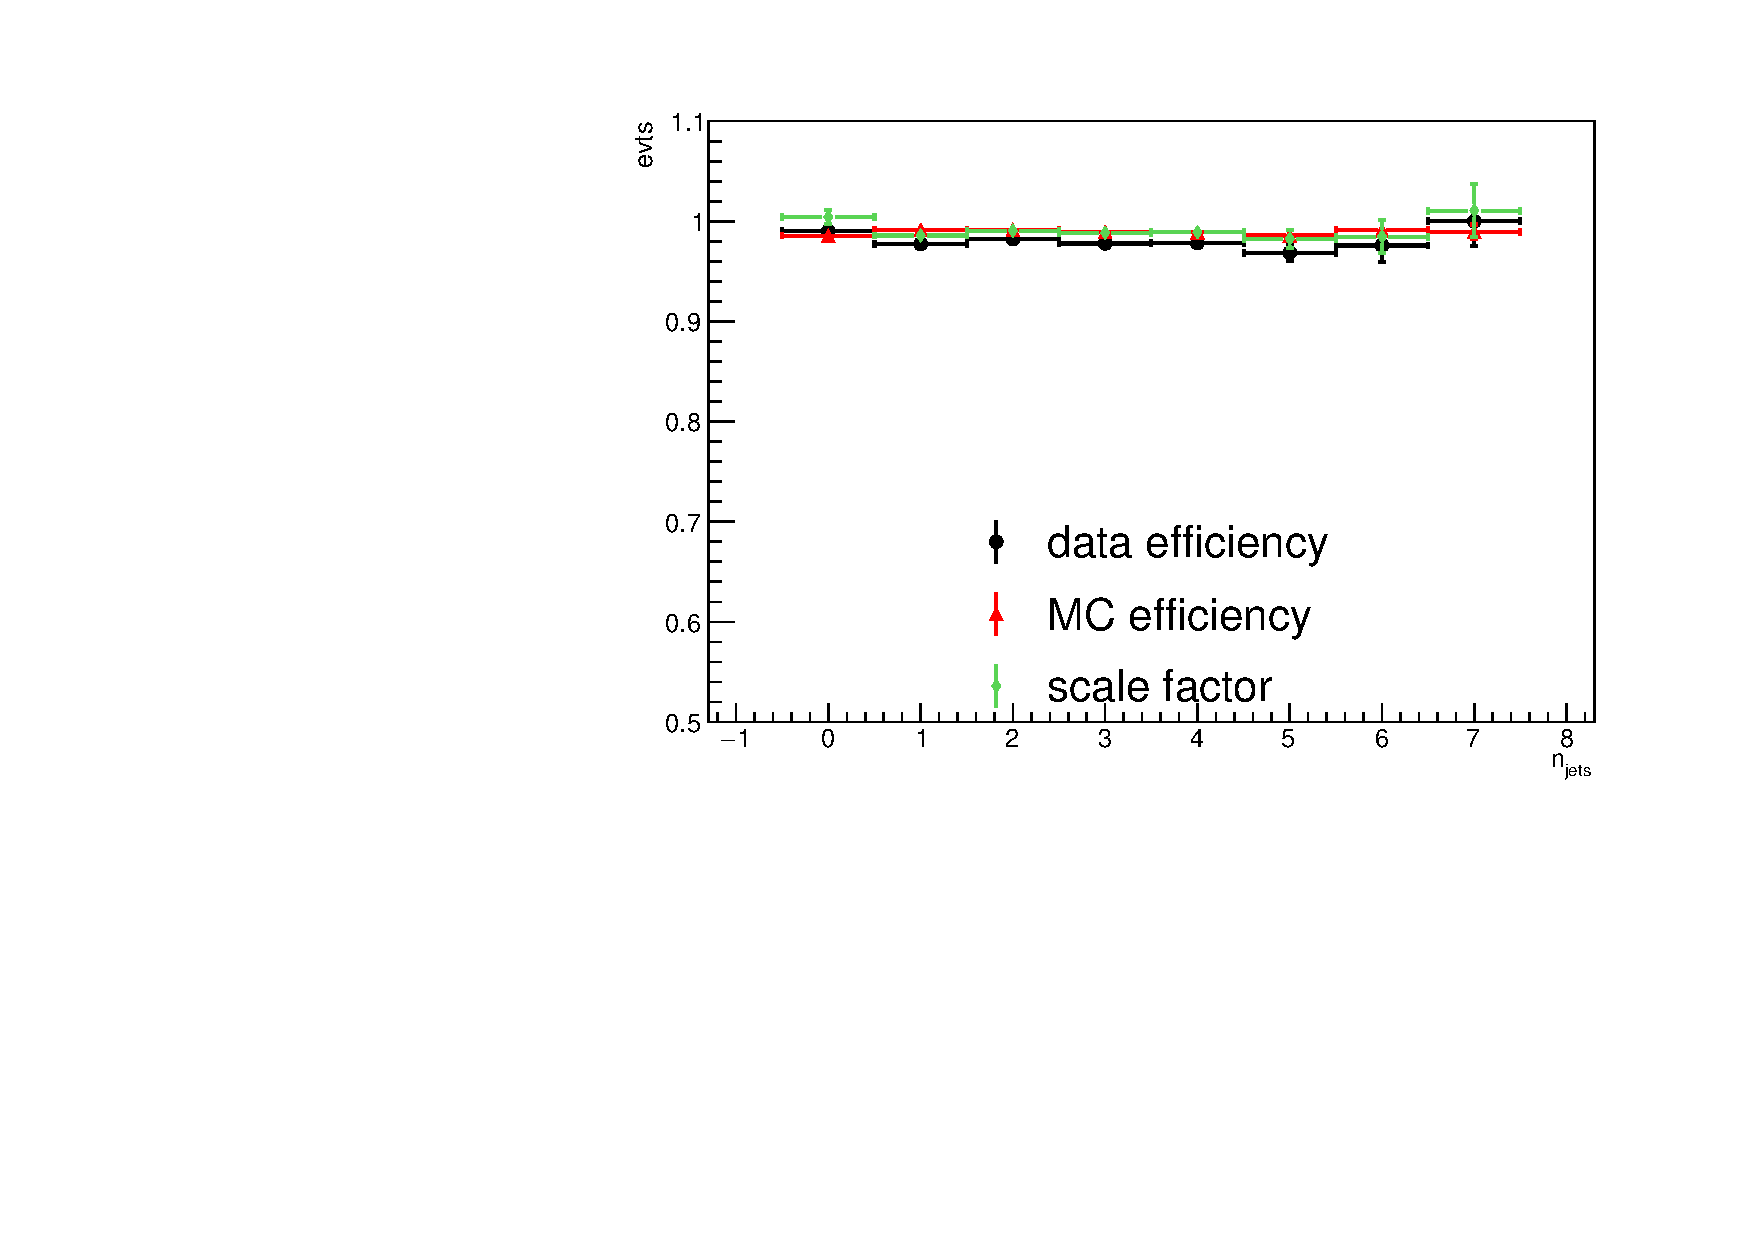
\includegraphics{Trigger/Figures/MET/ee/jet_multi}}
    \resizebox{0.48 \textwidth}{!}{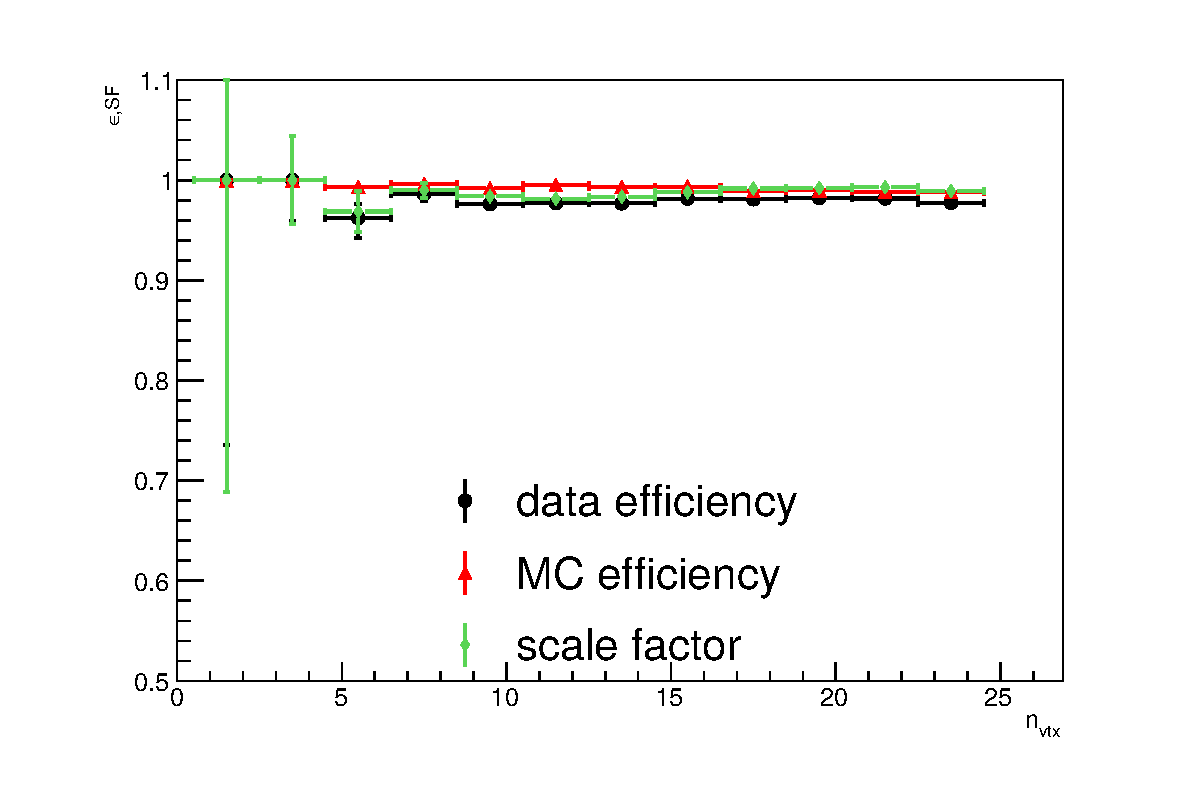
\includegraphics{Trigger/Figures/MET/ee/vertex_multi}}  
      \caption{Efficiencies of the trigger selection in the \ee channel for simulation and data and the corresponding scale factor. The upper row shows the efficiency as a function of $\eta$ of the leading (left) and subleading (right) electron. The middle row shows the efficiency as a function of \pt of the leading (left) and subleading (right) electron. The lower row shows the efficiency as a function of the jet multiplicity on the left and the vertex multiplicity on the right.
       The error bars indicate statistical uncertainties. }  
      
    \label{fig:MET_ee}
  \end{center}
\end{figure}

\begin{figure}[htbp!]
  \begin{center}
    \resizebox{0.48 \textwidth}{!}{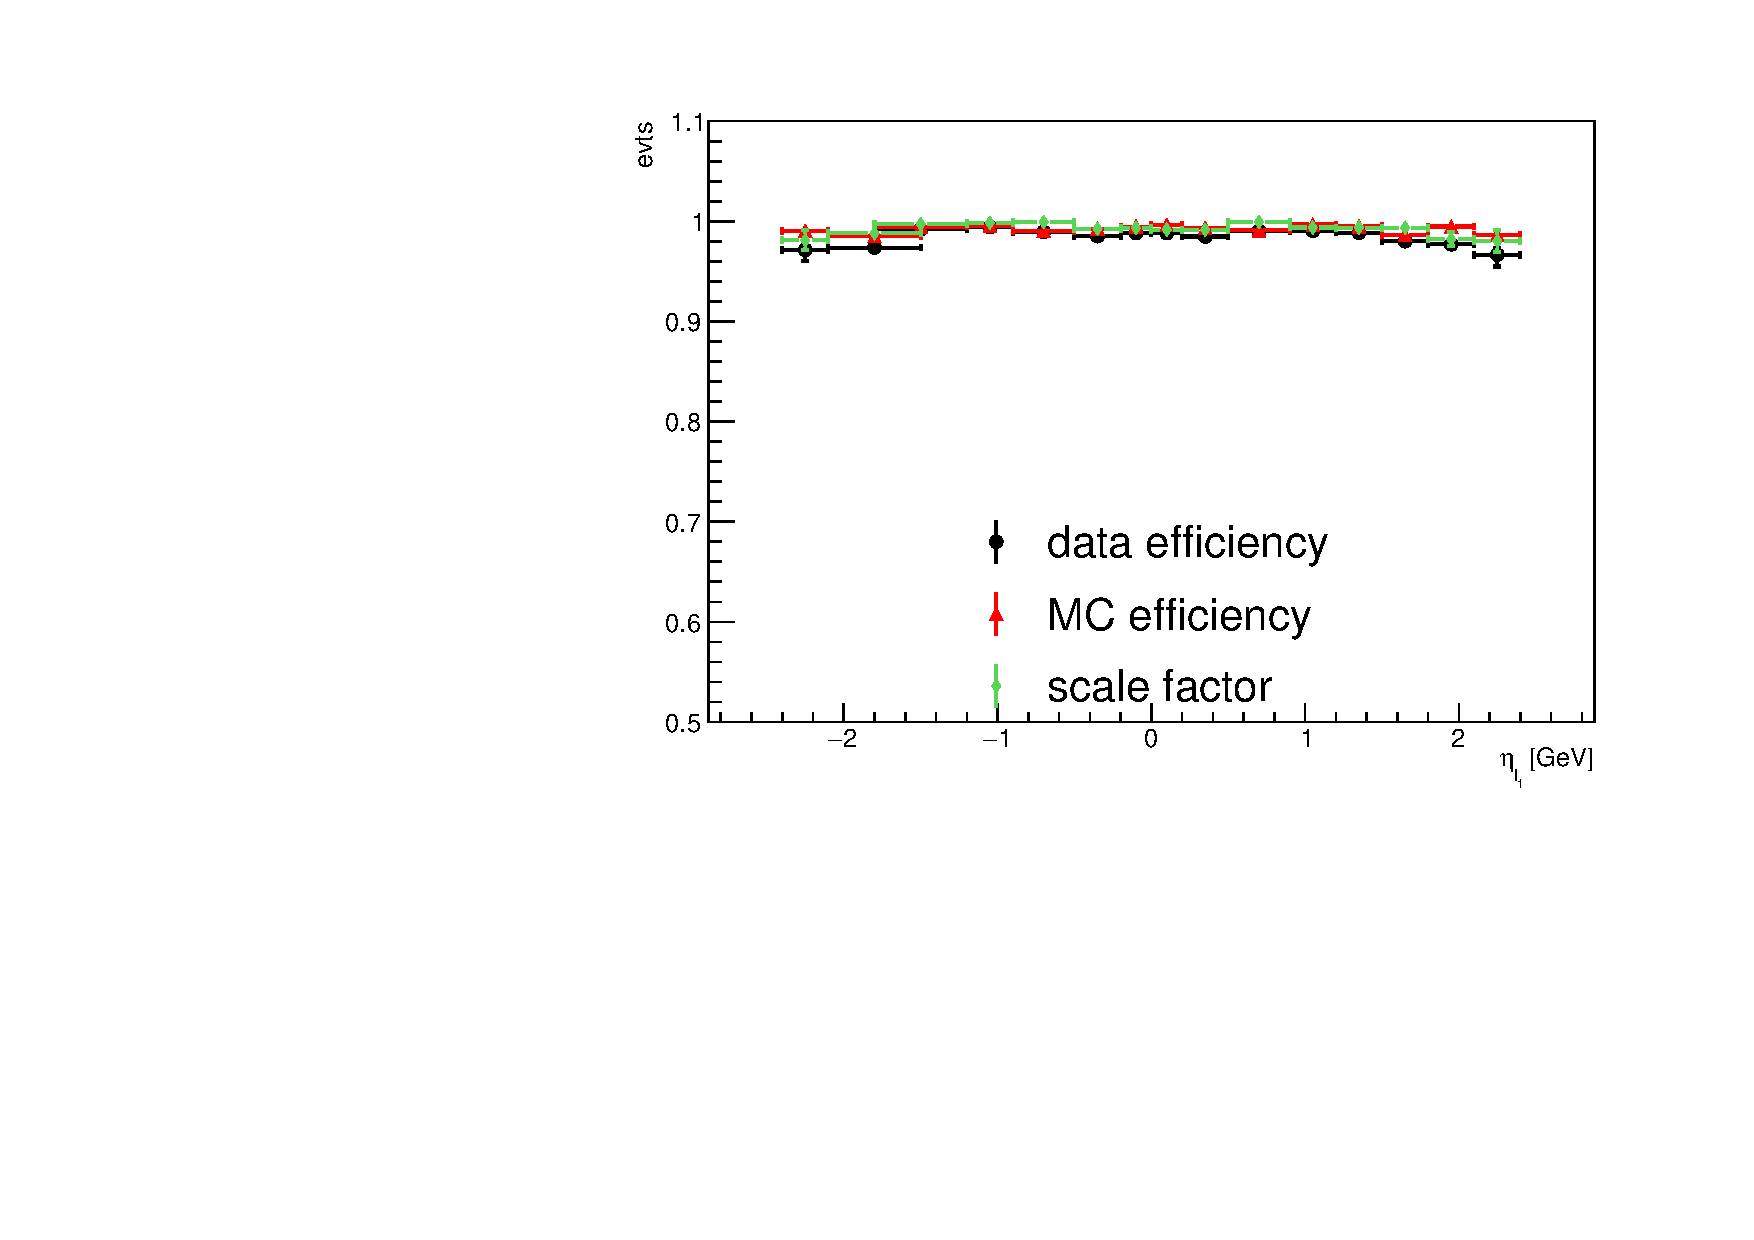
\includegraphics{Trigger/Figures/MET/mumu/leading_eta}}
    \resizebox{0.48 \textwidth}{!}{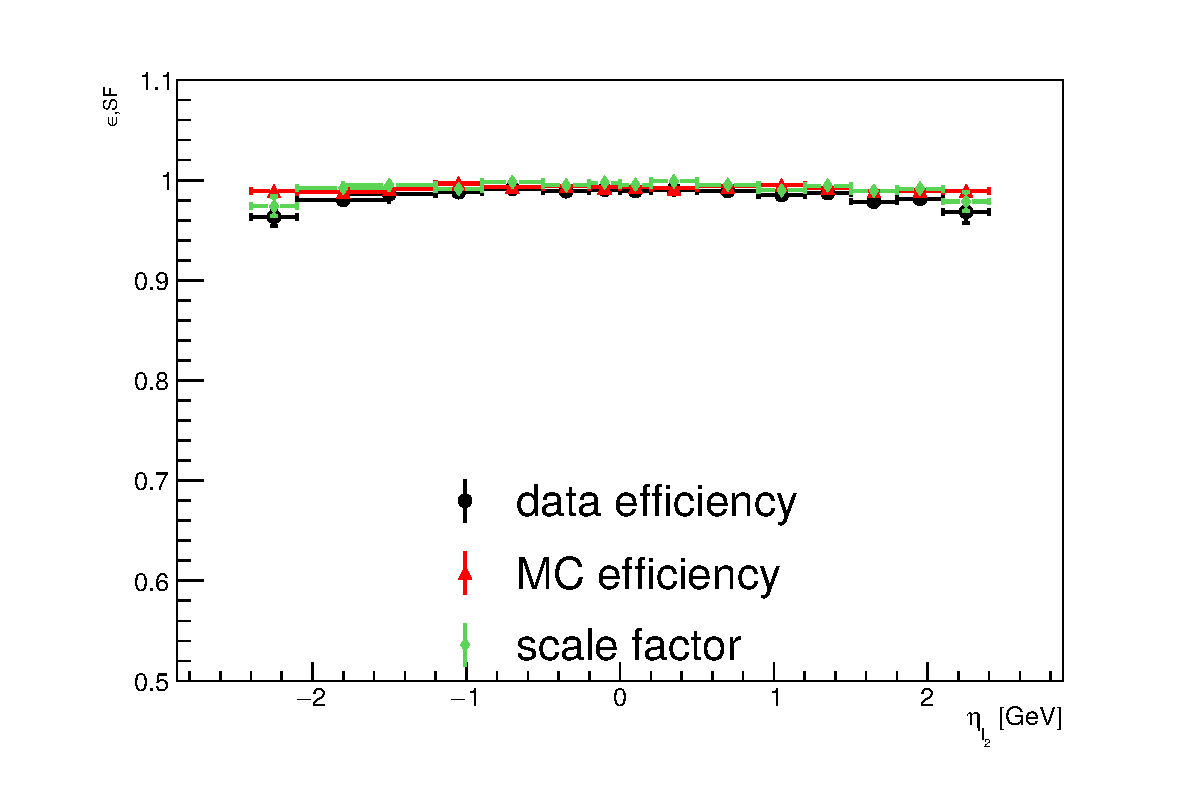
\includegraphics{Trigger/Figures/MET/mumu/seleading_eta}}
    \resizebox{0.48 \textwidth}{!}{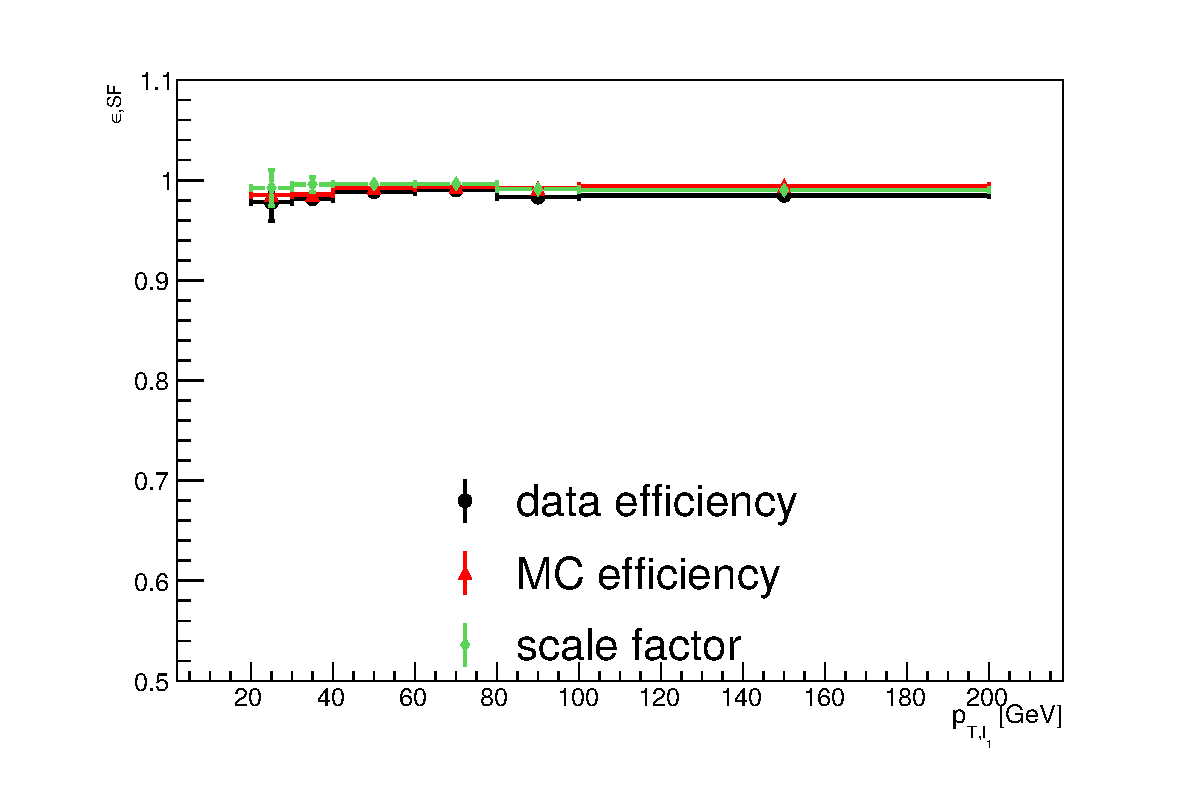
\includegraphics{Trigger/Figures/MET/mumu/leading_pt}}
    \resizebox{0.48 \textwidth}{!}{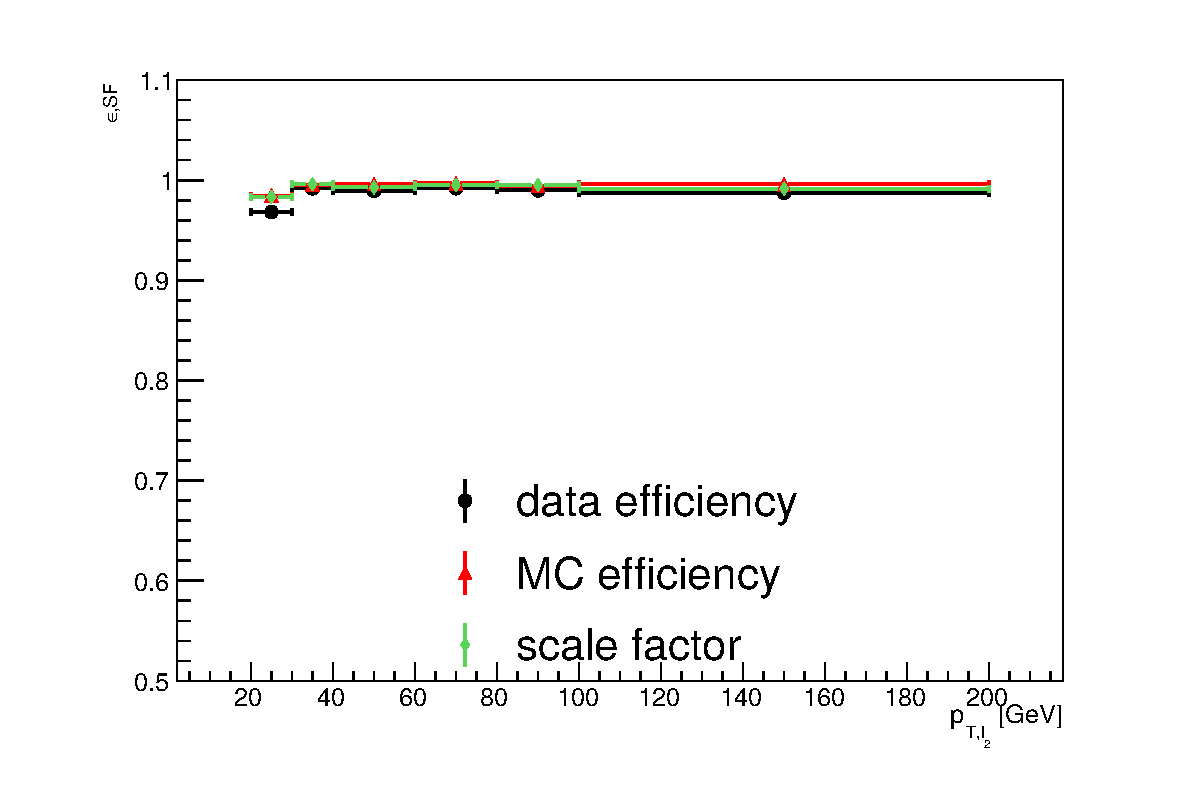
\includegraphics{Trigger/Figures/MET/mumu/seleading_pt}}
    \resizebox{0.48 \textwidth}{!}{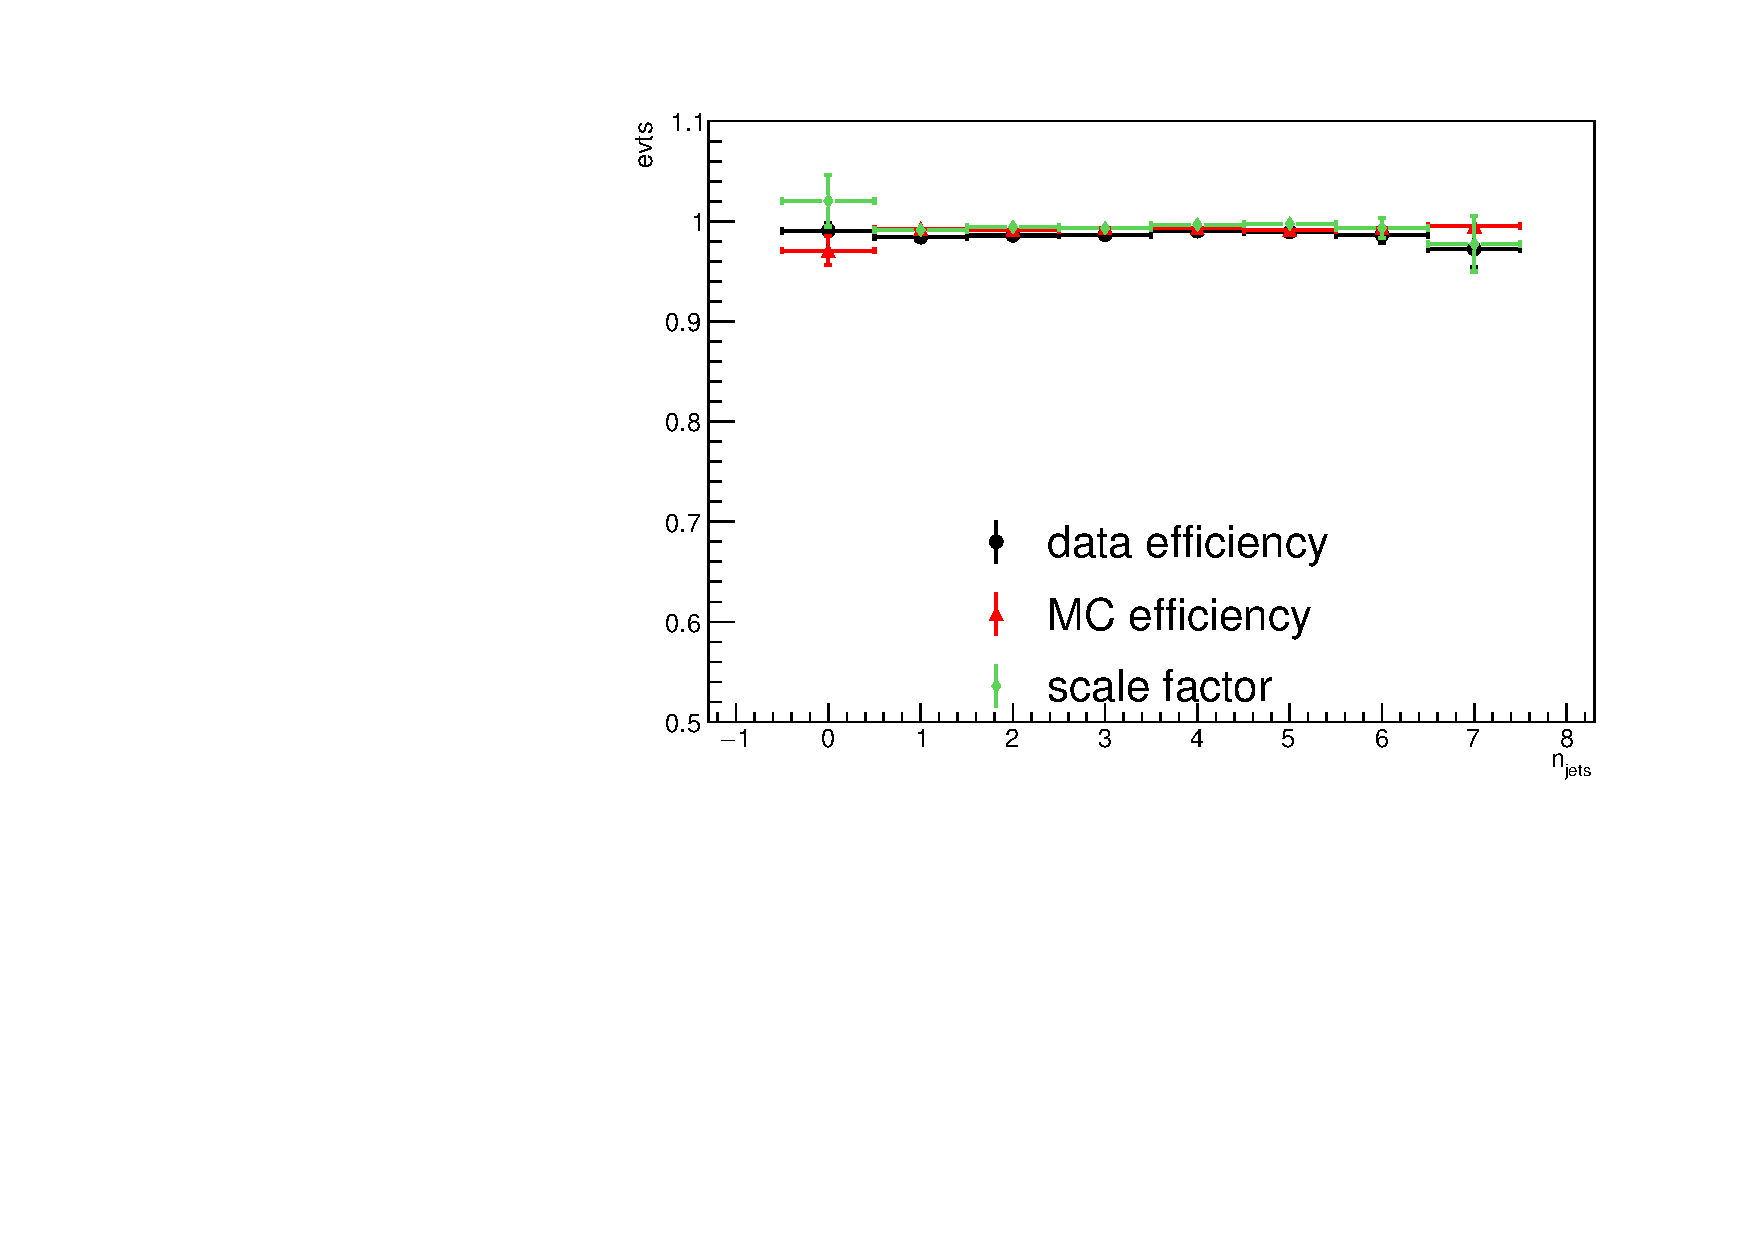
\includegraphics{Trigger/Figures/MET/mumu/jet_multi}}
    \resizebox{0.48 \textwidth}{!}{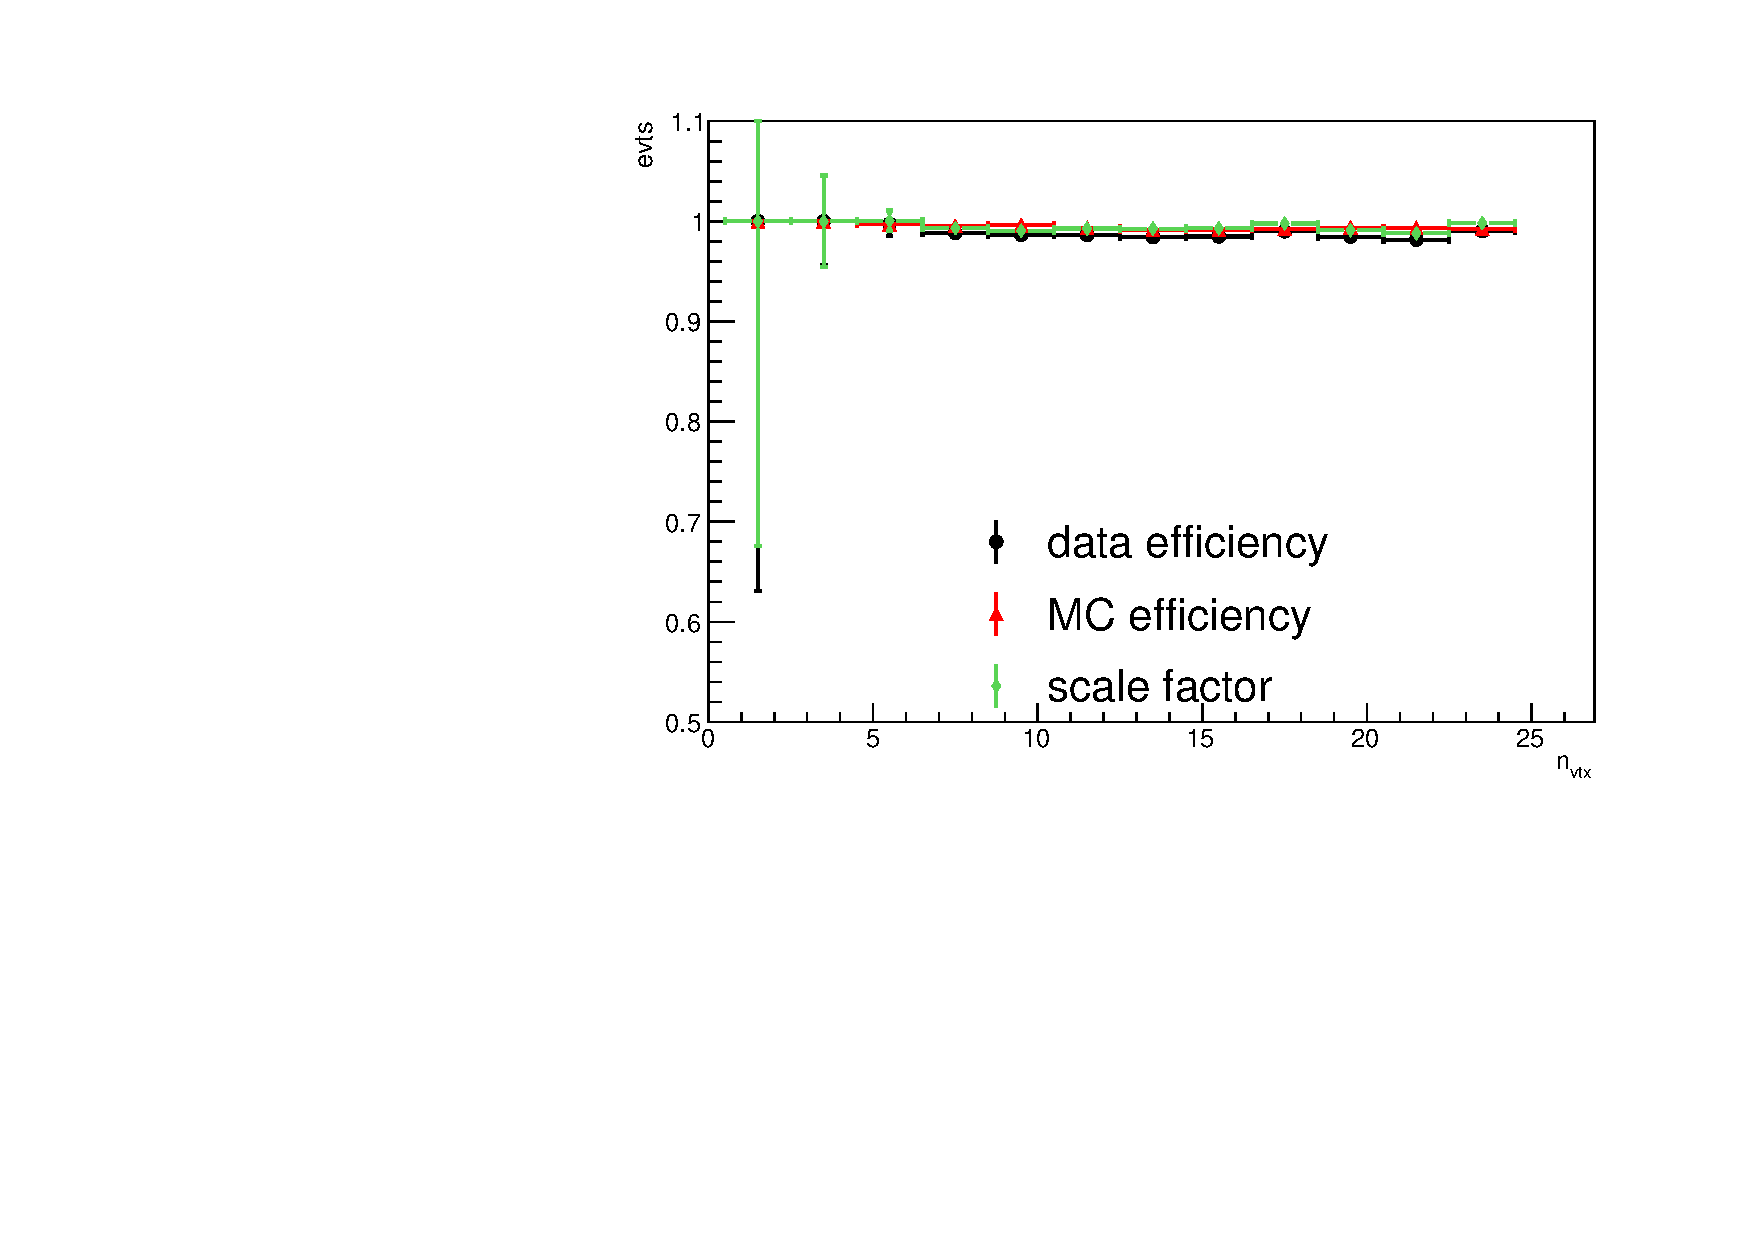
\includegraphics{Trigger/Figures/MET/mumu/vertex_multi}}  
      \caption{Efficiencies of the trigger selection in the \mumu channel for simulation and data and the corresponding scale factor. The upper row shows the efficiency as a function of $\eta$ of the leading (left) and subleading (right) lepton. The middle row shows the effciency as a function of \pt of the leading (left) and subleading (right) lepton. The lower row shows the efficiency as a function of the jet multiplicity on the left and the vertex multiplicity on the right.
      The error bars indicate statistical uncertainties. }  
      
    \label{fig:MET_mumu}
  \end{center}
\end{figure}

\begin{figure}[htbp!]
  \begin{center}
    \resizebox{0.48 \textwidth}{!}{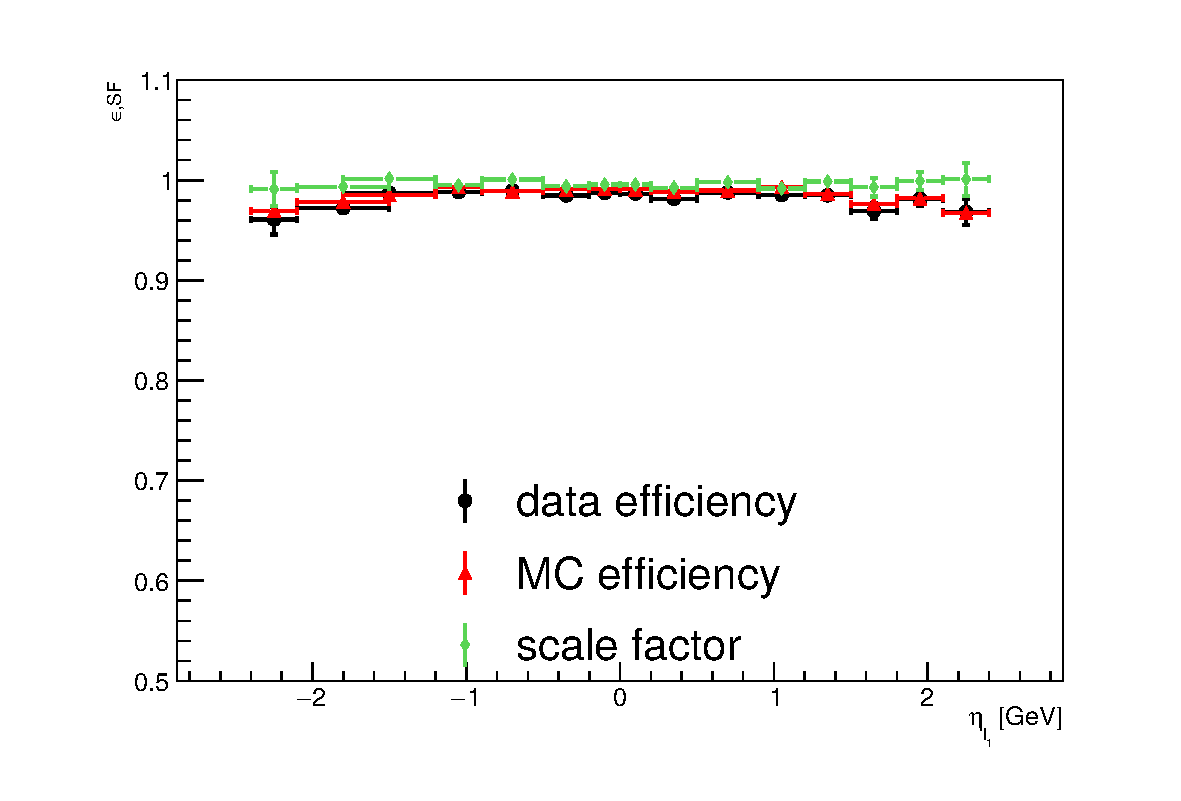
\includegraphics{Trigger/Figures/MET/emu/leading_eta}}
    \resizebox{0.48 \textwidth}{!}{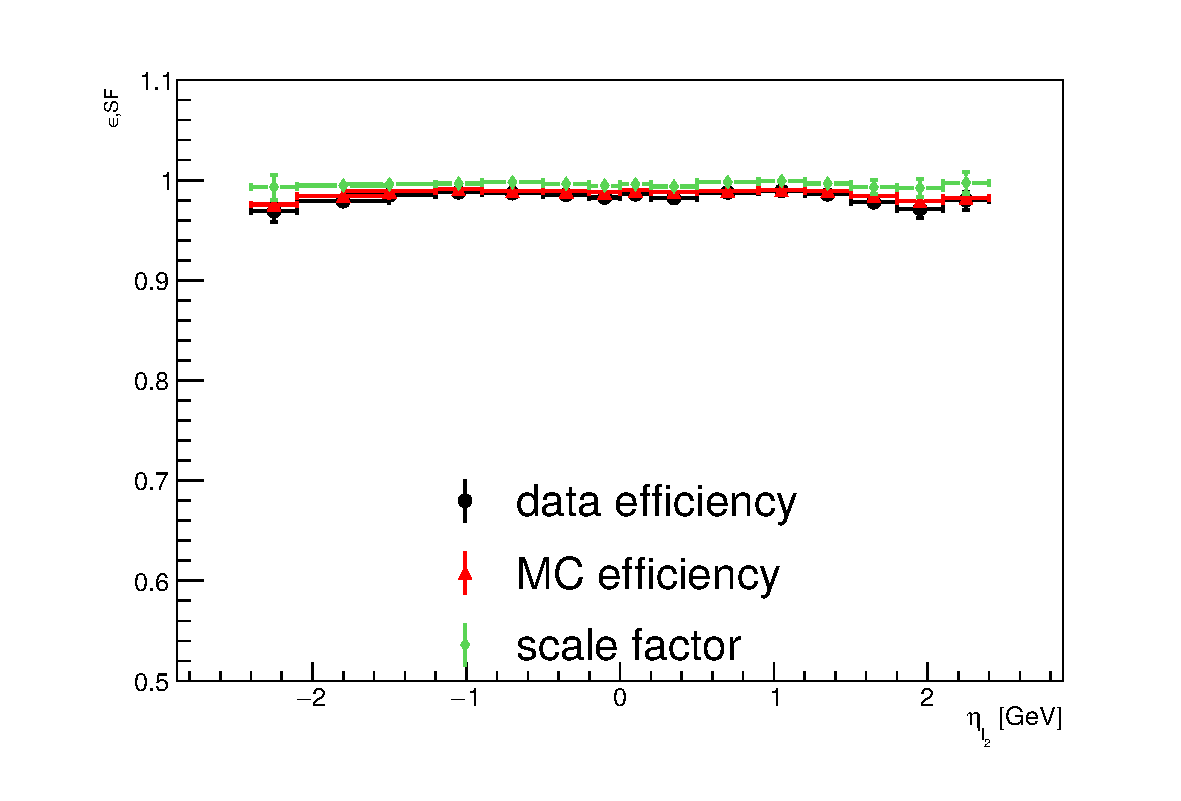
\includegraphics{Trigger/Figures/MET/emu/seleading_eta}}
    \resizebox{0.48 \textwidth}{!}{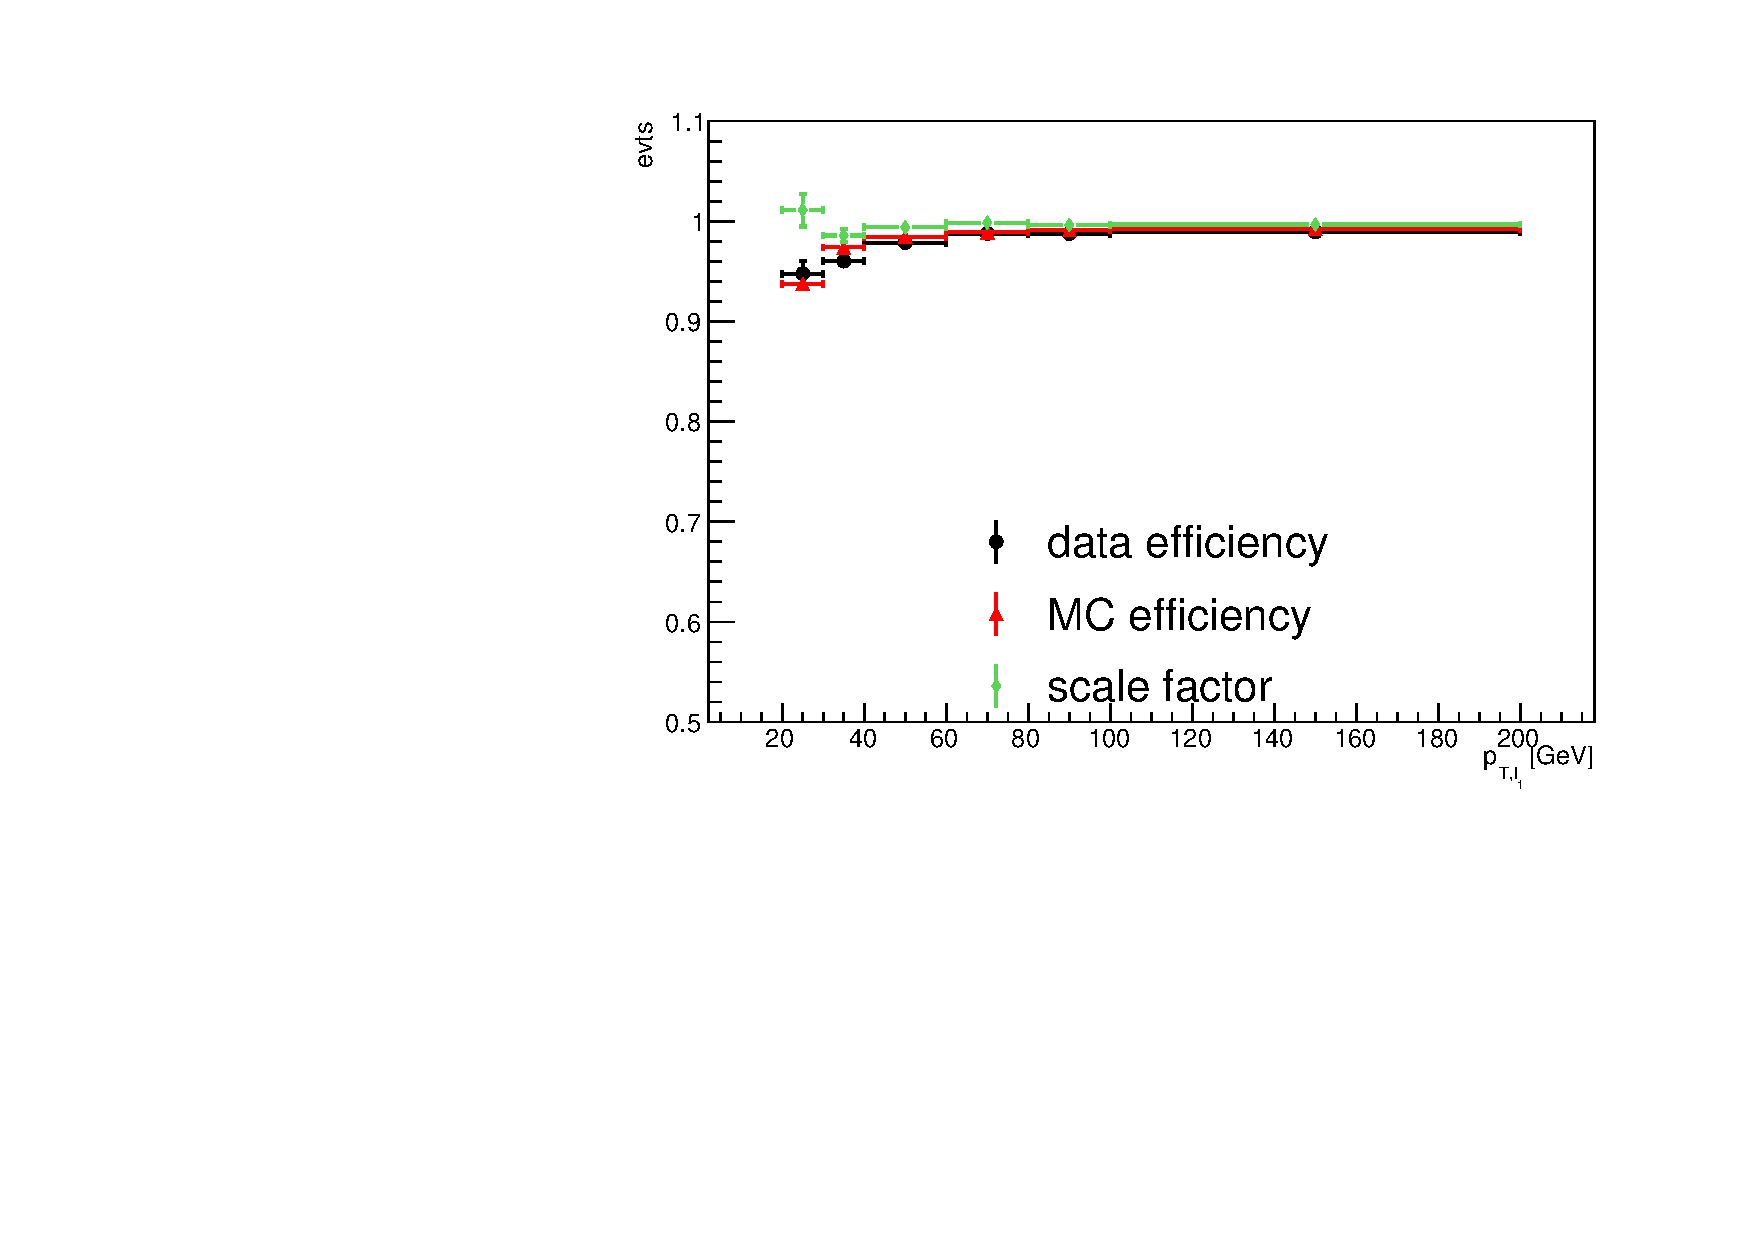
\includegraphics{Trigger/Figures/MET/emu/leading_pt}}
    \resizebox{0.48 \textwidth}{!}{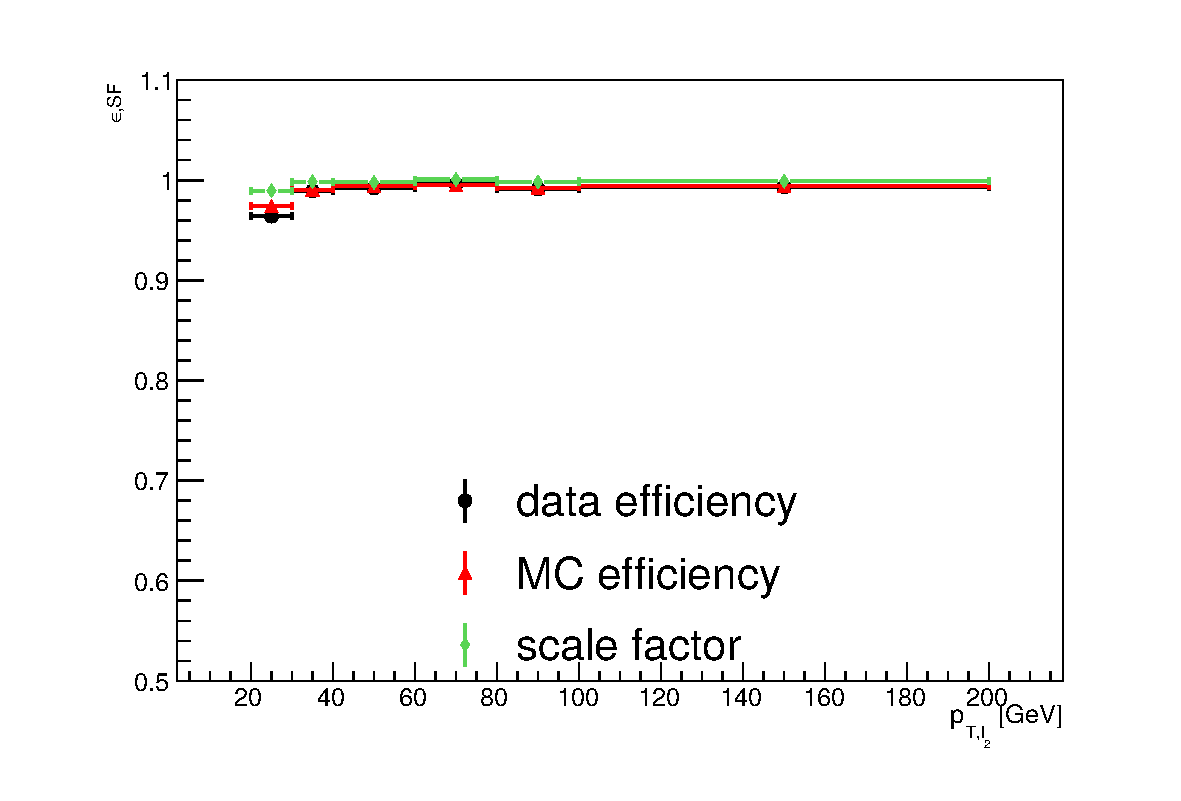
\includegraphics{Trigger/Figures/MET/emu/seleading_pt}}
    \resizebox{0.48 \textwidth}{!}{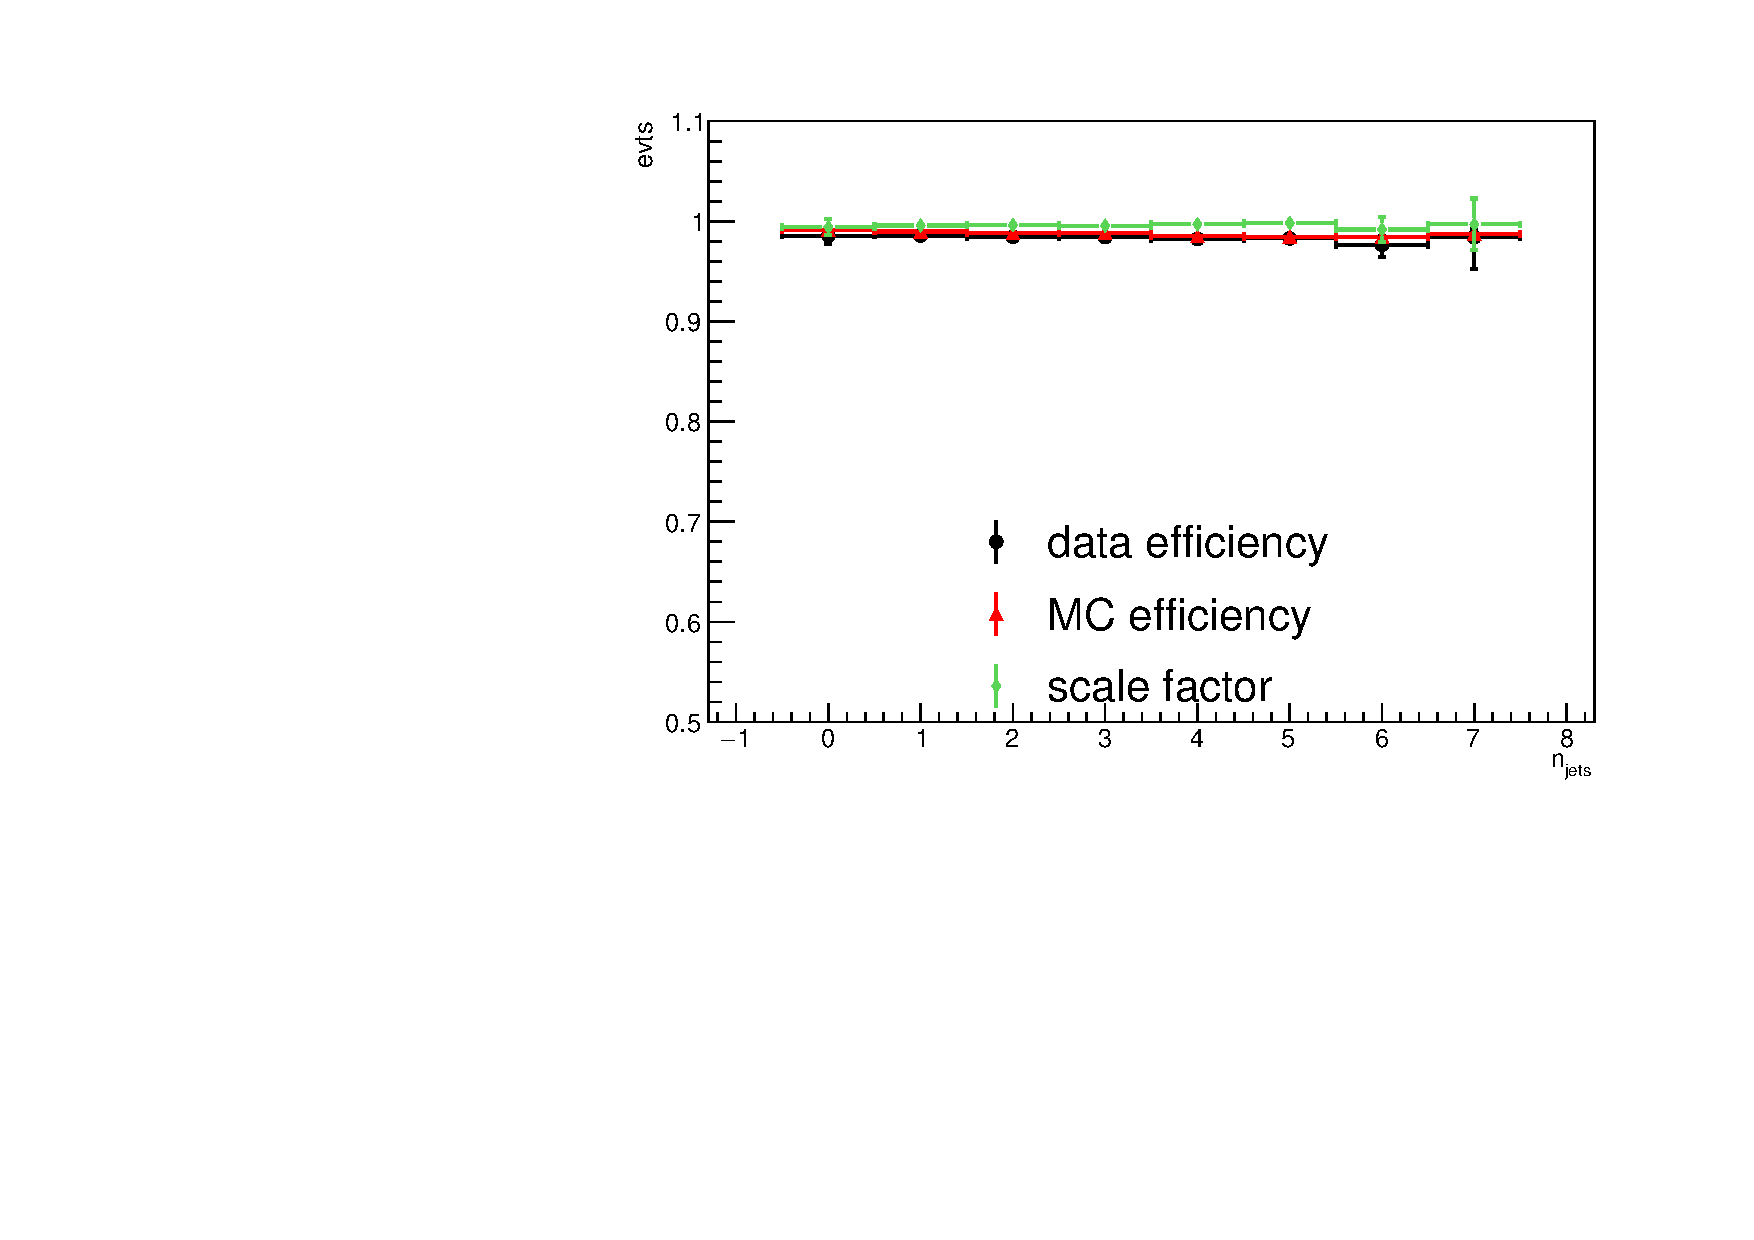
\includegraphics{Trigger/Figures/MET/emu/jet_multi}}
    \resizebox{0.48 \textwidth}{!}{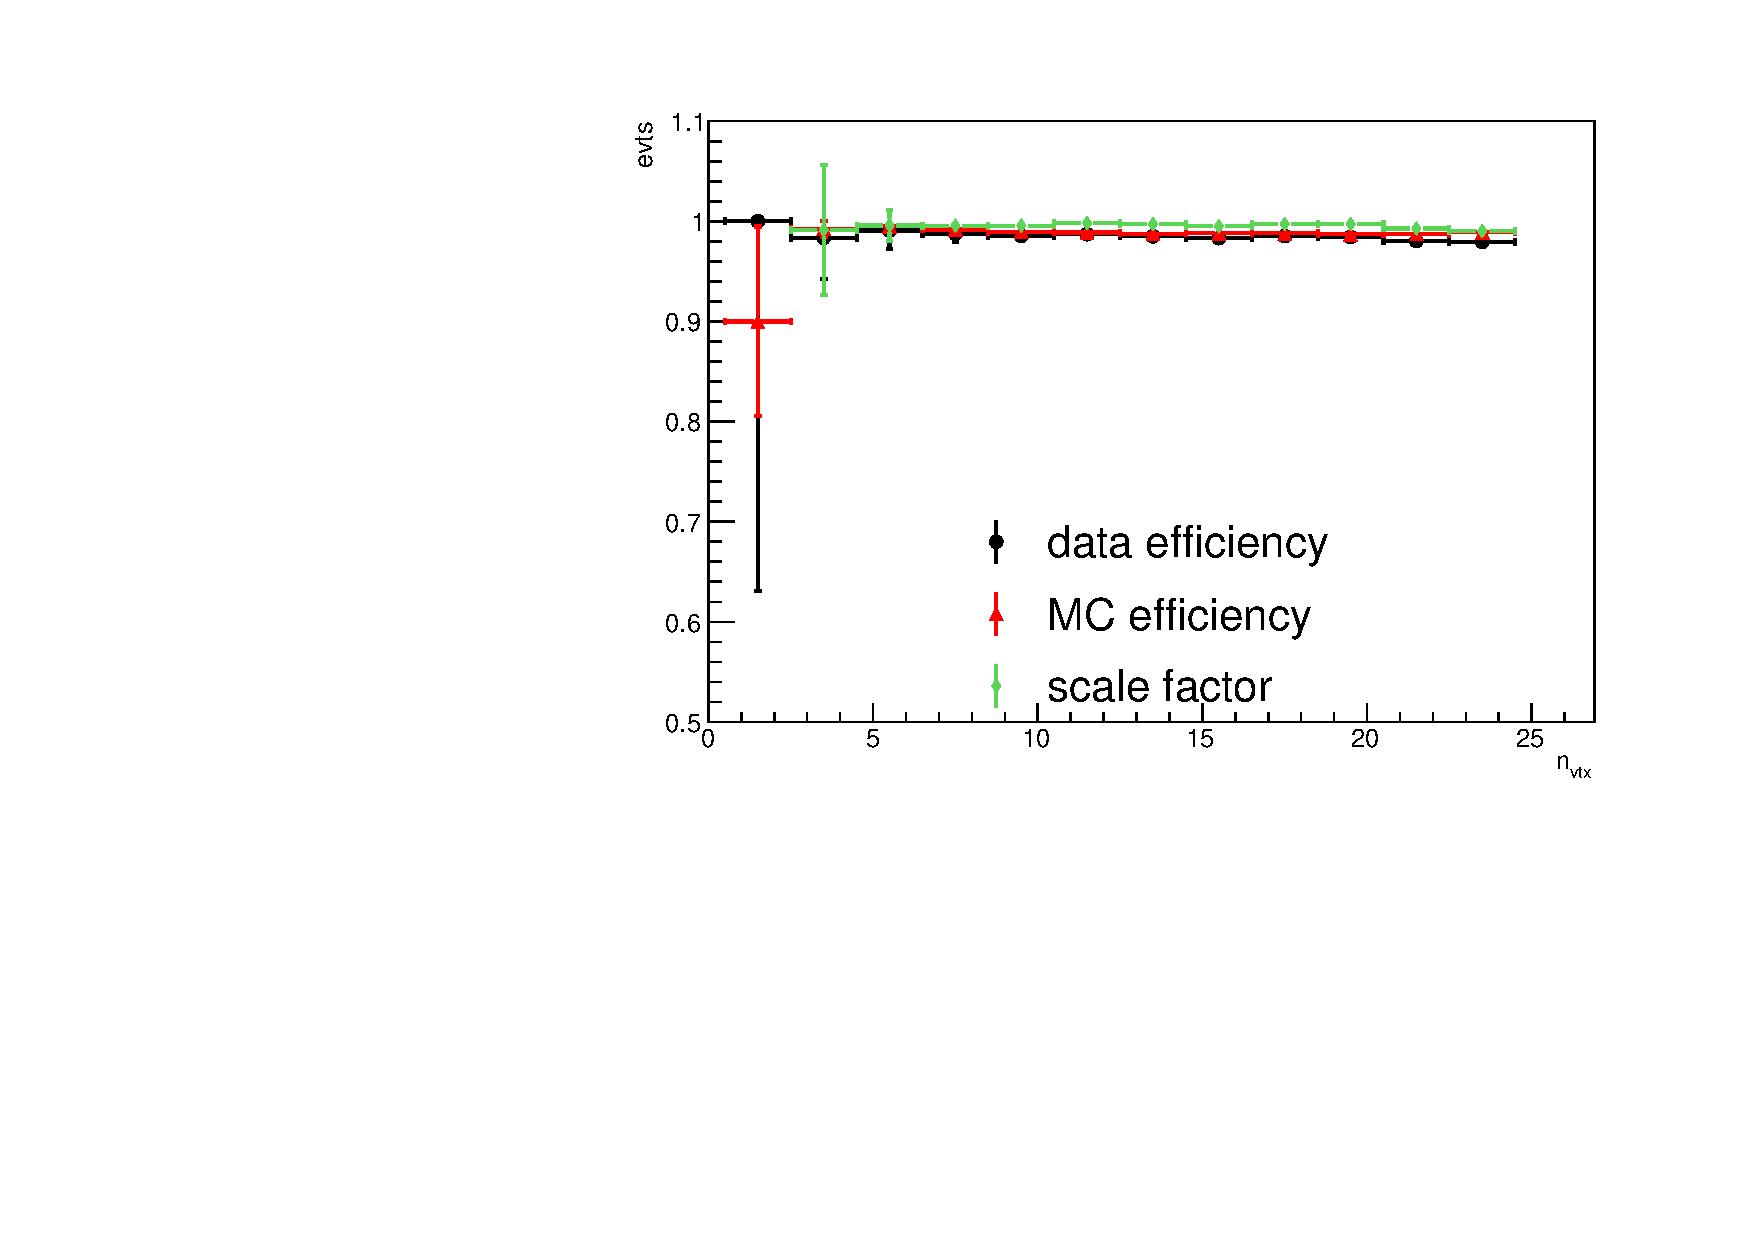
\includegraphics{Trigger/Figures/MET/emu/vertex_multi}}  
      \caption{Efficiencies of the trigger selection in the \emu channel for simulation and data and the corresponding scale factor. The upper row shows the efficiency as a function of $\eta$ of the leading (left) and subleading (right) muon. The middle row shows the effciency as a function of \pt of the leading (left) and subleading (right) muon. The lower row shows the efficiency as a function of the jet multiplicity on the left and the vertex multiplicity on the right.
      The error bars indicate statistical uncertainties. }  
      
    \label{fig:MET_emu}
  \end{center}
\end{figure}

The trigger efficiencies are shown as a function of \pt and $\eta$ of the leading and subleading electrons, the number of jets in the event, and the number of primary vertices. 
For the \ee channel (see Figure~\ref{fig:MET_ee}) the trigger efficiency is close to $100\%$ in most parts of the phase space and the efficiencies in data and simulation agree within uncertainties. The
efficiency shows small variations depending on the $\eta$ of the two electrons.
The small bins with a very low number of events around $|\eta| \approx 1.4$ correspond to a region of the detector where the electromagnetic calorimeter is not instrumented.
The trigger efficiency shows some dependence on the \pt of the leading electron, especially for $\pt<30\GeV$. The single lepton trigger has a requirement of $\pt \geq 27 \GeV$ which contributes to the \pt dependence.
The statistical uncertainty in the threshold region is large. The number of \ttbar events in that region is comparably low, so that the impact of the decreased efficiency for low \pt (also referred to as the turn-on of the trigger efficiency) is small. 
There is very little dependence of the trigger efficiency on the \pt of the subleading electron, due to the lower threshold in the dielectron trigger and the addition of the single-electron trigger.
The trigger efficiency does not depend on the number of jets, which is especially important for \ttbar events, which may contain a large amount of jets.
The number of primary vertices is an indication for the number of pile-up collisions in an event. The trigger efficiency does not depend on the number of vertices,
which shows that the impact of additional pileup collisions is small.

The trigger efficiency in the \mumu channel is close to $100\%$ and flat for most of the phase space (see Figure~\ref{fig:MET_mumu}). There are small variations of the efficiency depending on $\eta$ of the leading and subleading
muon. The efficiency also shows a small turn-on effect for the \pt of the subleading muon. Other variations are not statistically significant.

The trigger efficiency in the \emu channel is again very close to $100\%$ and efficiencies in data and simulation agree very well. There is a small drop in the efficiency for high $|\eta|$ for both the leading and the subleading lepton, but the agreement between data and simulation shows that detector effects are well modeled.
Similar to the efficiency in the \ee channel the efficiency decreases for $\pt < 30 \GeV$, likely due to the behavior of the electron triggers.
The trigger efficiency is flat against the number of jets and primary vertices.

Overall the trigger efficiency is close to $100\%$ for all three channels. The simulation generally agrees with the data, leading to scale factors that are close to unity.

For the \emu data set, the efficiency of the single-lepton triggers can also be measured from data sets selected with a trigger for a single lepton of a different flavor. The electron trigger efficiency can be measured in a data set selected with a single-muon trigger and vice versa.
These events closely correspond to the events selected for the \ttbar cross section measurement.
This method cannot be used for the measurement of dilepton trigger efficiencies, since there are not enough events that contain three leptons.
The method can be used to check the \ETm based trigger efficiency measurement by comparing the single lepton trigger efficiency obtained with both methods, as shown in Section~\ref{sec:TriggerComp}.

\section{Method using tag-and-probe}  %Section - 1.3 
\label{sec:TriggerTPMethod}

The tag-and-probe method provides an alternative trigger efficiency measurement that is independent from the measurement described in the last section.
In a tag-and-probe measurement, the trigger efficiency is measured independently in data and simulation by using the decay of a Z boson into two leptons.

In general, one of the leptons (the tag) is required to pass a tight selection. This selection includes matching the offline lepton to the lepton reconstructed at trigger level by requiring them to have a minimal distance and difference in \pt. The second lepton (the probe) is only required to pass the lepton selection later used in the \ttbar cross section measurement (see Section~\ref{sec:xsec_sel}). The invariant mass of the two leptons then needs to be within the Z boson mass window, in which case it is assumed that the leptons are real leptons.
The probe can either pass the trigger requirement for the trigger that is to measured ("passing probe") or fail it ("failing probe"). The efficiency is then determined by dividing the number of passing probes by the number of all probes.

Even in the region of the Z boson mass a background of pairs with at least one fake lepton remains. This residual fake lepton contamination is determined by fitting distributions for real leptons (signal) and fake leptons (background) to the invariant mass of the dilepton system. The fit is done for both passing and failing probes. The background is often described by an exponential function. The signal has a more complicated functional form and can for example be parametrized by a double Voigtian function. The Voigtian function is a convolution of a Lorentz and a Gaussian function. When the trigger efficiency is measured in data it is also possible to fit templates from MC. This can allow a better modeling of detector effects that are included in the simulation.
The trigger efficiency in simulation is often measured for a background-free sample (pure Drell-Yan sample). In these cases a fit is not needed and it is sufficient to count the number of passing and failing probes.

The efficiency is measured differentially as a function of kinematic properties of the lepton. The measurement is performed independently in each bin of the distribution.
It commonly depends on both the $\eta$ and the \pt of the lepton. 

In contrast to the efficiency measurement using orthogonal triggers (see Section~\ref{sec:TriggerMetMethod}), the tag-and-probe measurement depends on a specific lepton. It measures the efficiency for each lepton, consequently several measurements have to be combined for a multilepton trigger or an efficiency measurement with multiple triggers (see Section~\ref{sec:TriggerComp}). 

Examples for the efficiency measurement in one bin as well as the overall scale factor for the muon part ("muon leg") of the Mu23\_TrkIsoVVL\_Ele12\_CaloIdL\_TrackIdL\_IsoVL trigger both for data and simulation and the resulting overall scale factors are shown in Figure~\ref{fig:TP_Mu23}. The fits are successful in modeling the \mll \; distribution for passing and failing probes in both data and simulation. The scale factor being close to unity shows that the simulation mostly reproduces the behavior in data.

\begin{figure}[htbp!]
  \begin{center}
    \resizebox{0.65 \textwidth}{!}{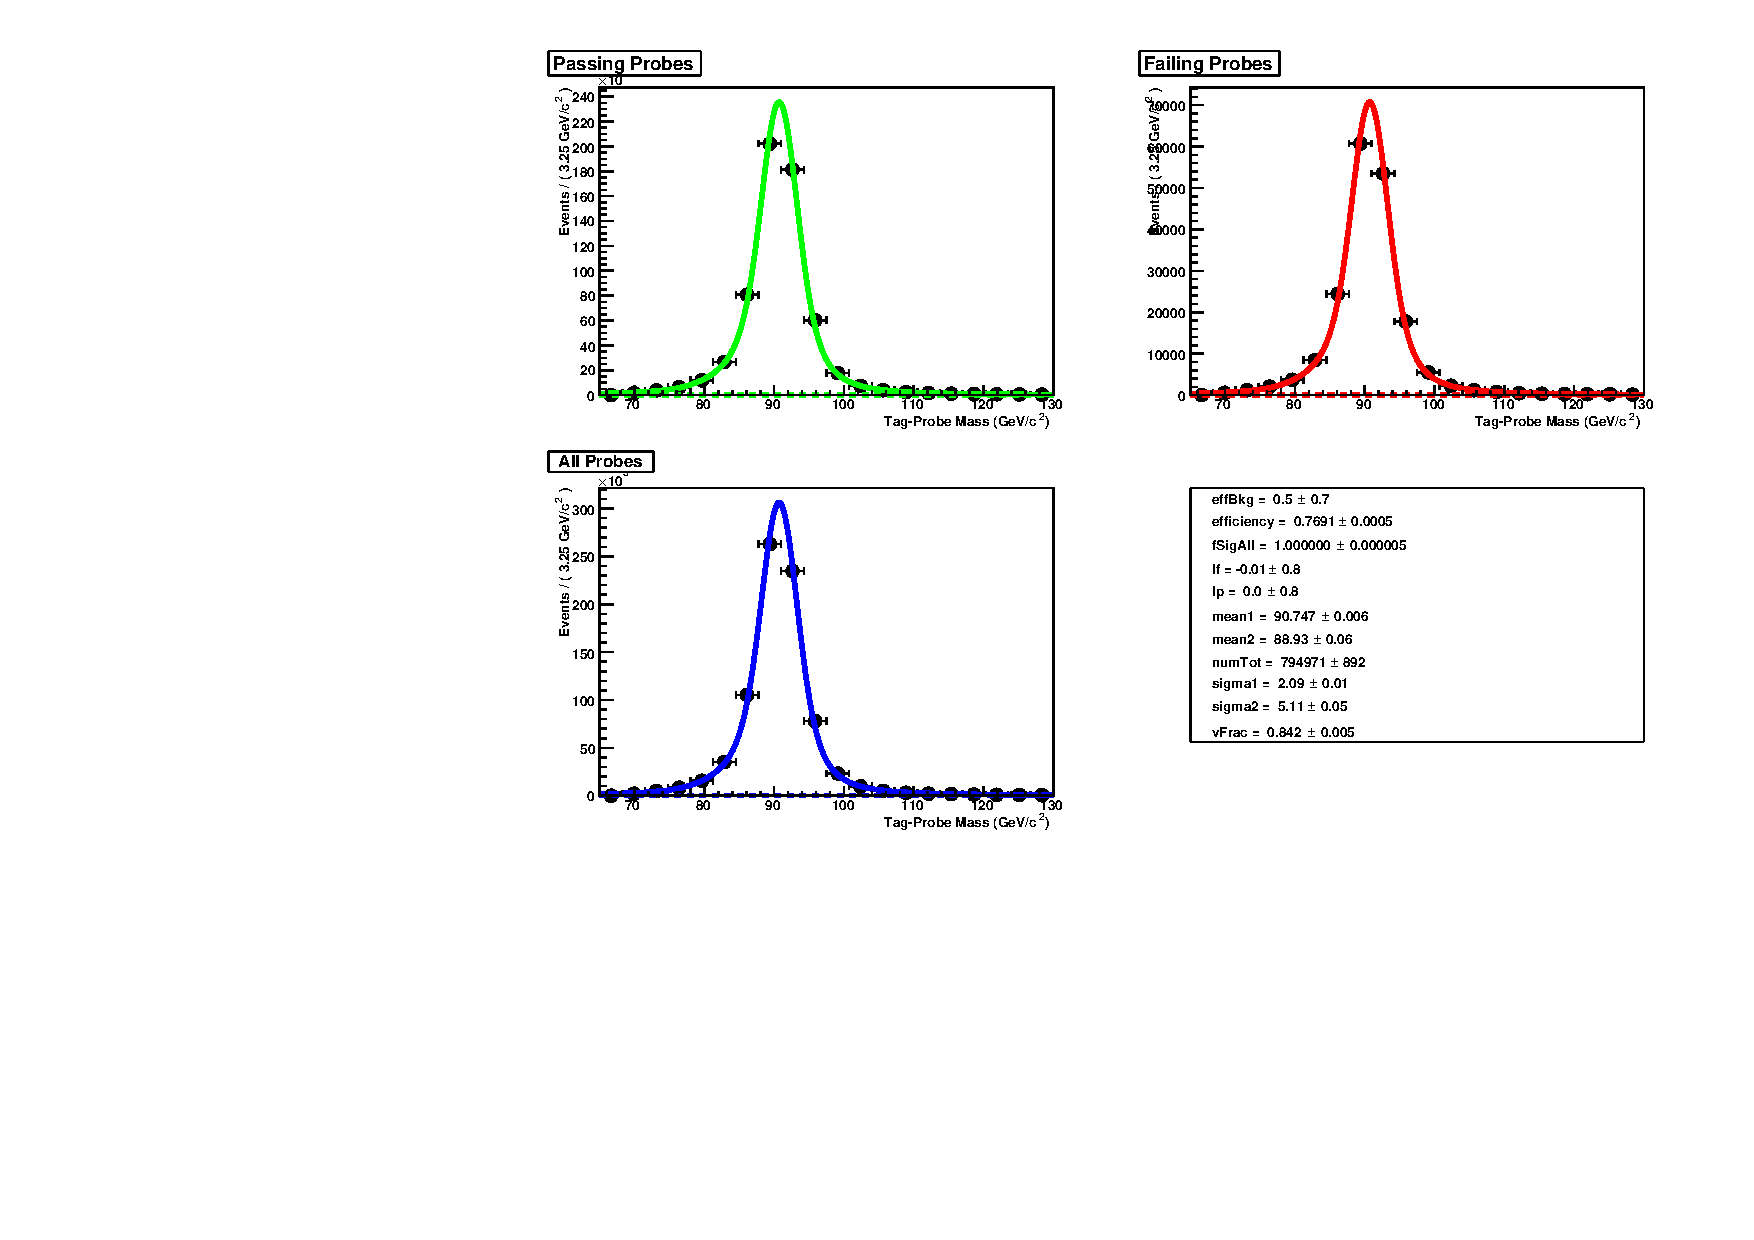
\includegraphics{Trigger/Figures/TaP/Mu23_data_fits}}
    \resizebox{0.65 \textwidth}{!}{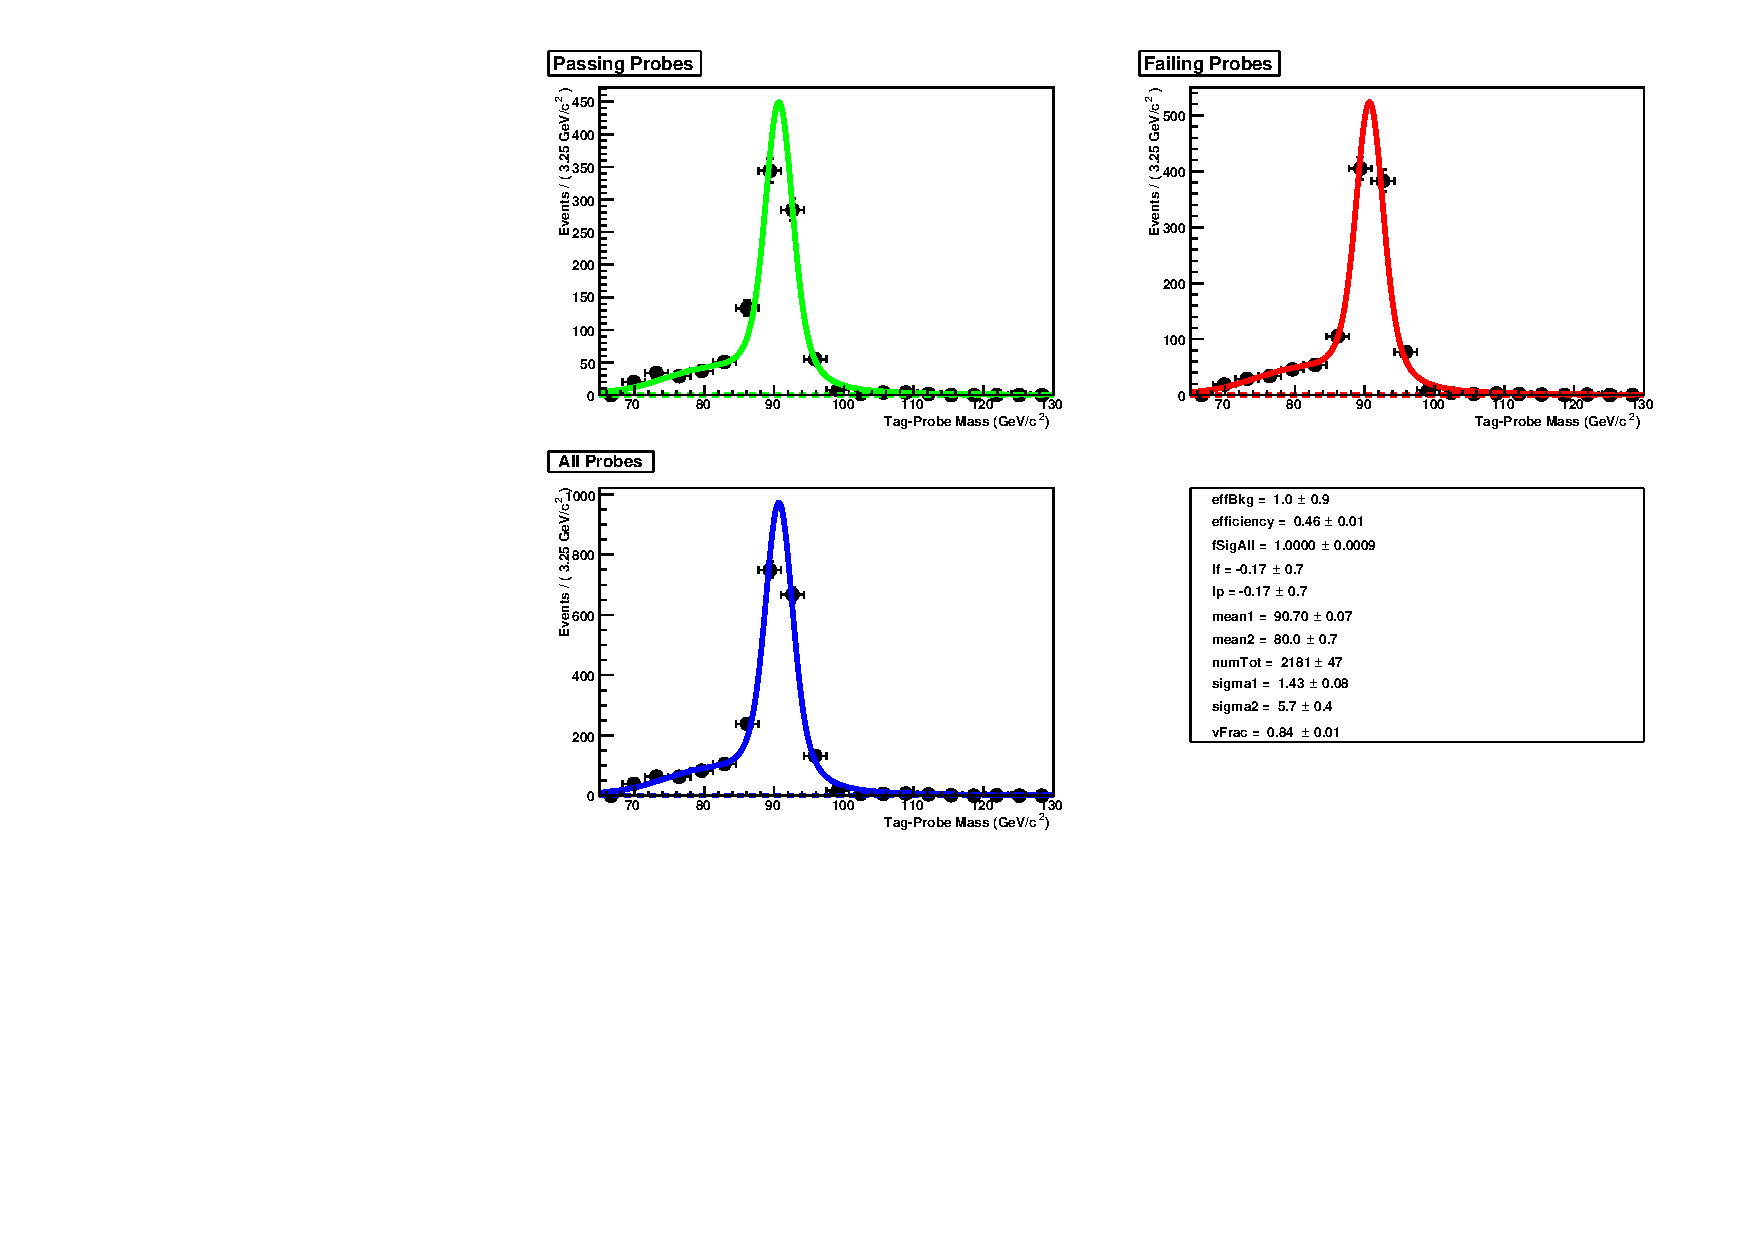
\includegraphics{Trigger/Figures/TaP/Mu23_MC_fits}}\\
    \resizebox{0.65 \textwidth}{!}{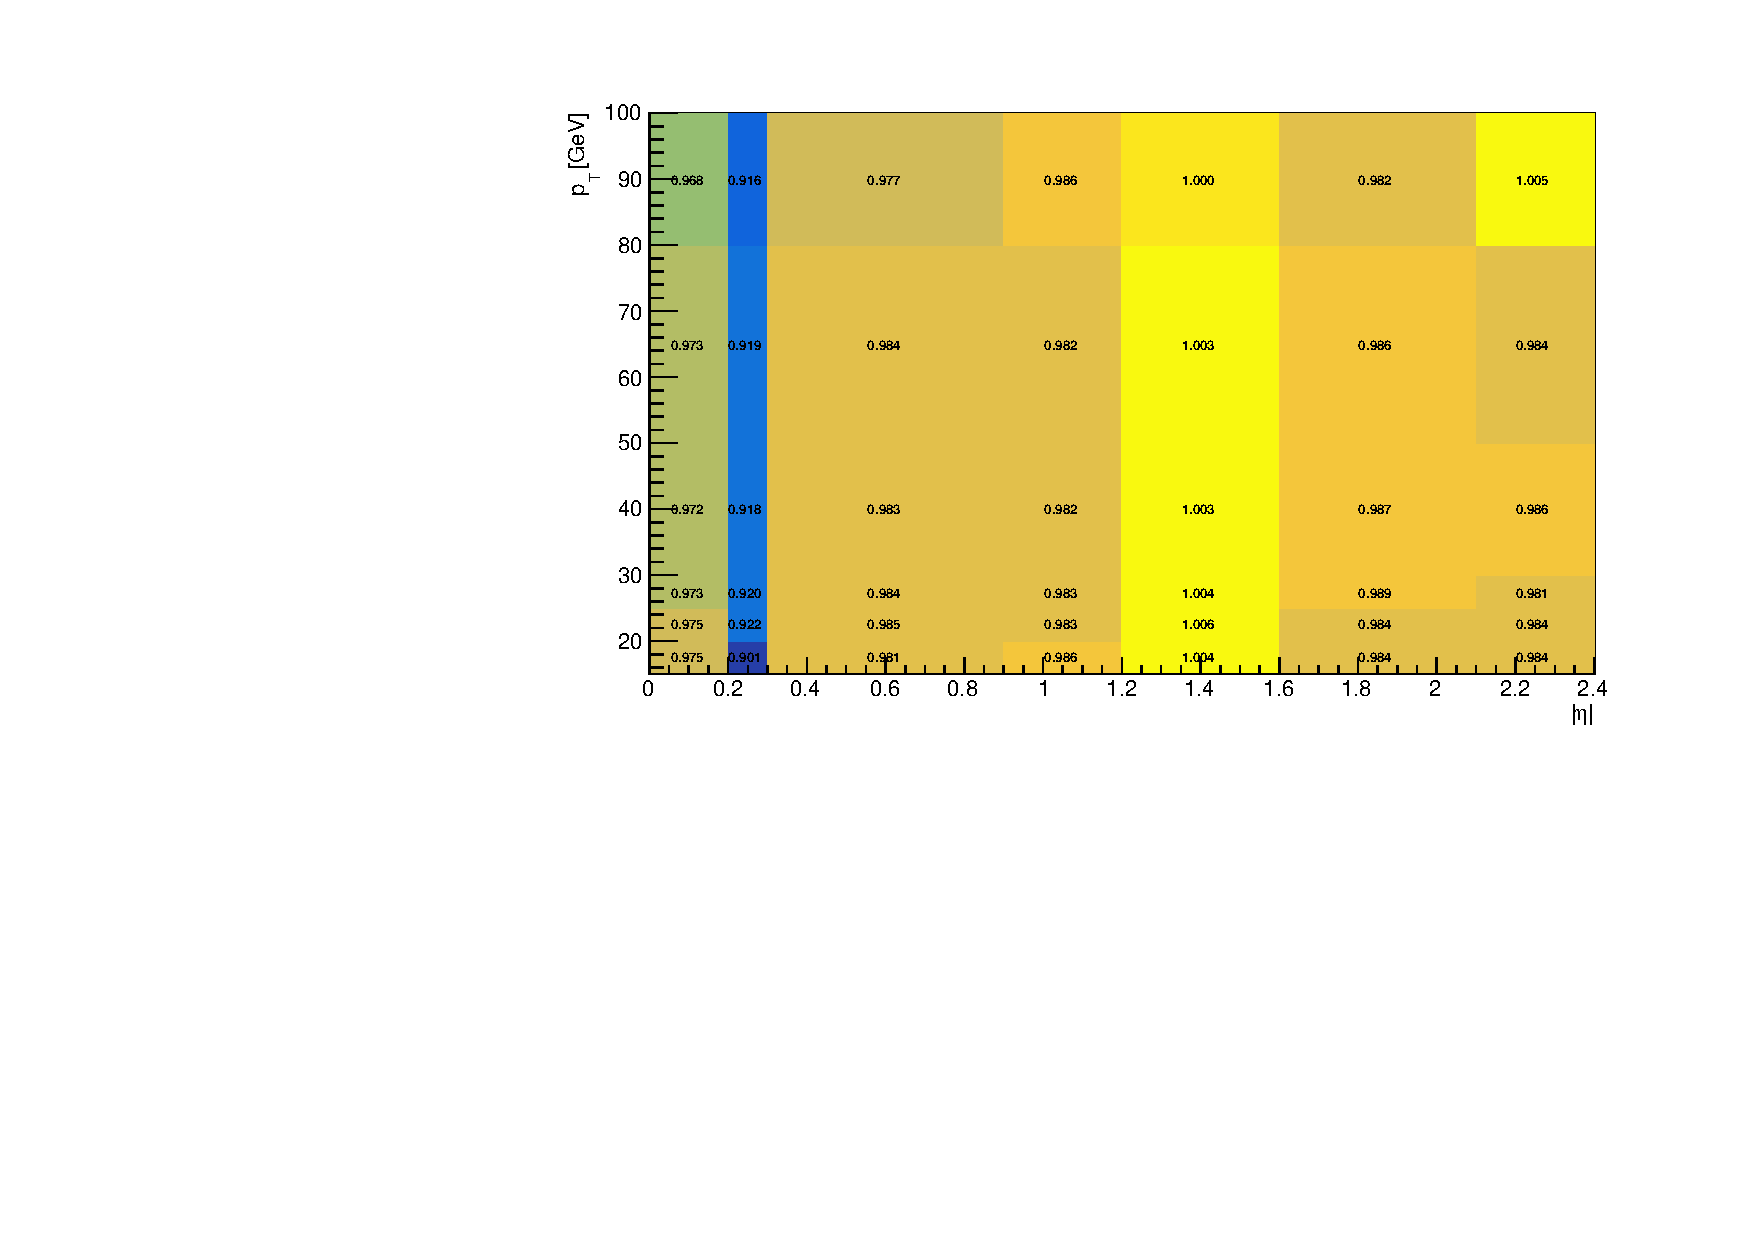
\includegraphics{Trigger/Figures/TaP/Mu23_sf}}
      \caption{Results of the trigger efficiency measurement with the tag-and-probe method for the Mu23 trigger leg. The four upper figures show the measurement for one bin for data  while the middle four figures show the same for simulation. The lower figure shows 
       the scale factor between data and simulation binned in $\eta$ and \pt. }  
    \label{fig:TP_Mu23}
  \end{center}
\end{figure}


Figure~\ref{fig:TP_Ele23} shows the efficiency measurement for the electron part ("electron leg") of the\\ Mu8\_TrkIsoVVL\_Ele23\_CaloIdL\_TrackIdL\_IsoVL trigger.
The fit is performed for passing and failing probes in data, while the efficiency in simulation is measured without a fit by counting the events in the Z boson mass peak.
The fits are successful and the efficiency in data and simulation agree within a few percent.

\begin{figure}[htbp!]
  \begin{center}
    \resizebox{0.6 \textwidth}{!}{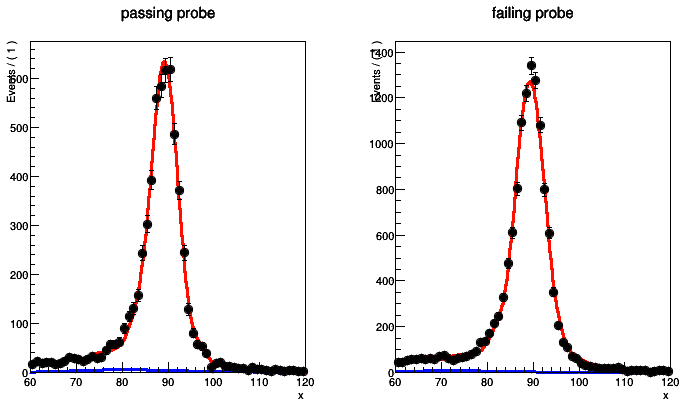
\includegraphics{Trigger/Figures/TaP/ele_plots_only}}
    \resizebox{0.39 \textwidth}{!}{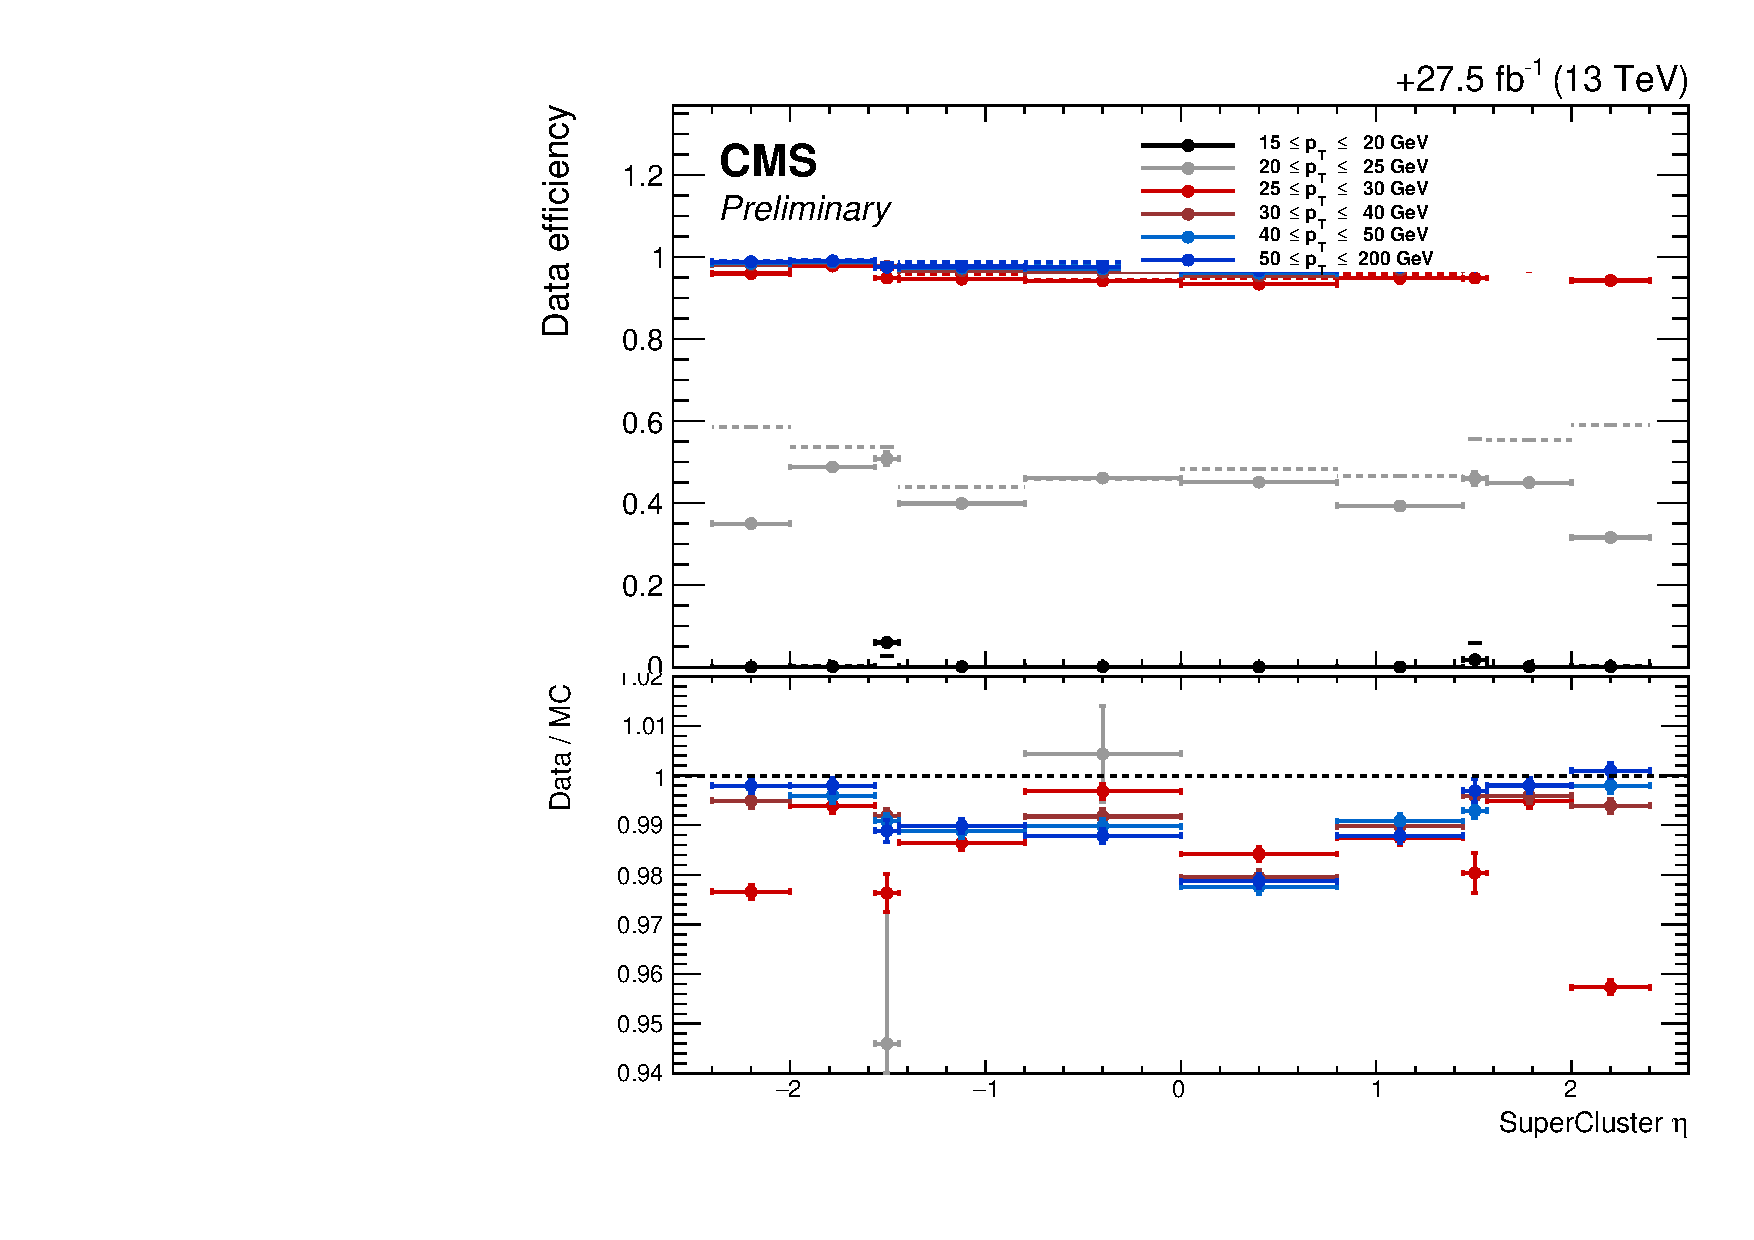
\includegraphics{Trigger/Figures/TaP/Ele23_data_eff}}
      \caption{Results of the trigger efficiency measurement with the tag-and-probe method for the Ele23 trigger leg. In the left figure the fit for one example bin in data is shown. The right figure shows the efficiency in data and simulation in bins of $\eta$ with multiple colored graphs showing the \pt dependence. In the lower panel the scale factors are shown in the same format. }  
    \label{fig:TP_Ele23}
  \end{center}
\end{figure}

The trigger efficiency for each of the two leptons in the dilepton trigger is combined and compared to the trigger efficiency measured with independent triggers in the next section.

%********************************************** Fourth Section


\section{Comparison of trigger efficiency measurements}
\label{sec:TriggerComp}

In order to assess the systematic uncertainty of the trigger efficiency measurement, the three methods described in Sections~\ref{sec:TriggerMetMethod} and~\ref{sec:TriggerTPMethod} are compared.
The independent trigger method measures the trigger efficiency mostly in \ttbar events, while the tag-and-probe method uses Z boson decays. The comparison consequently covers two 
very different phase spaces and serves as a good estimation of the systematic uncertainty.

The comparison of the independent trigger and the tag-and-probe methods has to contend with one fundamental difference: the independent trigger method using \ETm triggers measures the trigger efficiency for a complete trigger selection (multiple triggers) and per event, defined by the existence of two isolated leptons fulfilling the kinematic cuts. In contrast, the tag-and-probe method measures the trigger efficiency for each lepton of each trigger separately. 

These per-leg efficiencies are combined to the efficiency for each dilepton trigger. This is done by multiplying the efficiencies of the single trigger legs, considering them to be uncorrelated. 
Next, the efficiencies of each of the lepton triggers ($\mathrm{trig}_A$ and $\mathrm{trig}_B$) involved in the trigger selection need to be combined. Since they are combined with a logical OR, this is done by multiplying the inefficiencies of the two triggers:

\begin{equation}
\epsilon(\mathrm{trig}_{combined}) = 1- (1-\epsilon(\mathrm{trig}_A))\cdot(1- \epsilon(\mathrm{trig}_B)).
\label{eq:TPcombine}
\end{equation}

The combined trigger efficiency measured with the tag-and-probe method can be applied per event for the complete trigger selection. It can then be compared to the trigger efficiency measured with the independent \ETm triggers.
For this comparison, both efficiencies are applied to scale the same simulated \ttbar sample. These \ttbar events are required to contain an electron and a muon (as described for the event selection in Section~\ref{sec:xsec_sel}) and the trigger efficiency scale factors are applied depending on the $\eta$ of these leptons.
After the rescaling, properties of these two sets of \ttbar events are compared as shown in Figure~\ref{fig:Clos_emu}.

The distributions are consistent with each other in nearly the whole phase space. The largest disagreement is found for events with electrons with $\pt<20\GeV$, but these events are not considered in the final event selection. This agreement shows that there is no systematic difference between the two methods, when measuring a trigger efficiency in the \ttbar phase space. This does not necessarily apply to any other possible phase space, but the trigger efficiency measurement here specifically applies to the \ttbar phase space. This agreement is considered for the determination of the systematic uncertainties on the trigger efficiency.

\begin{figure}[htbp!]
  \begin{center}
    \resizebox{0.48 \textwidth}{!}{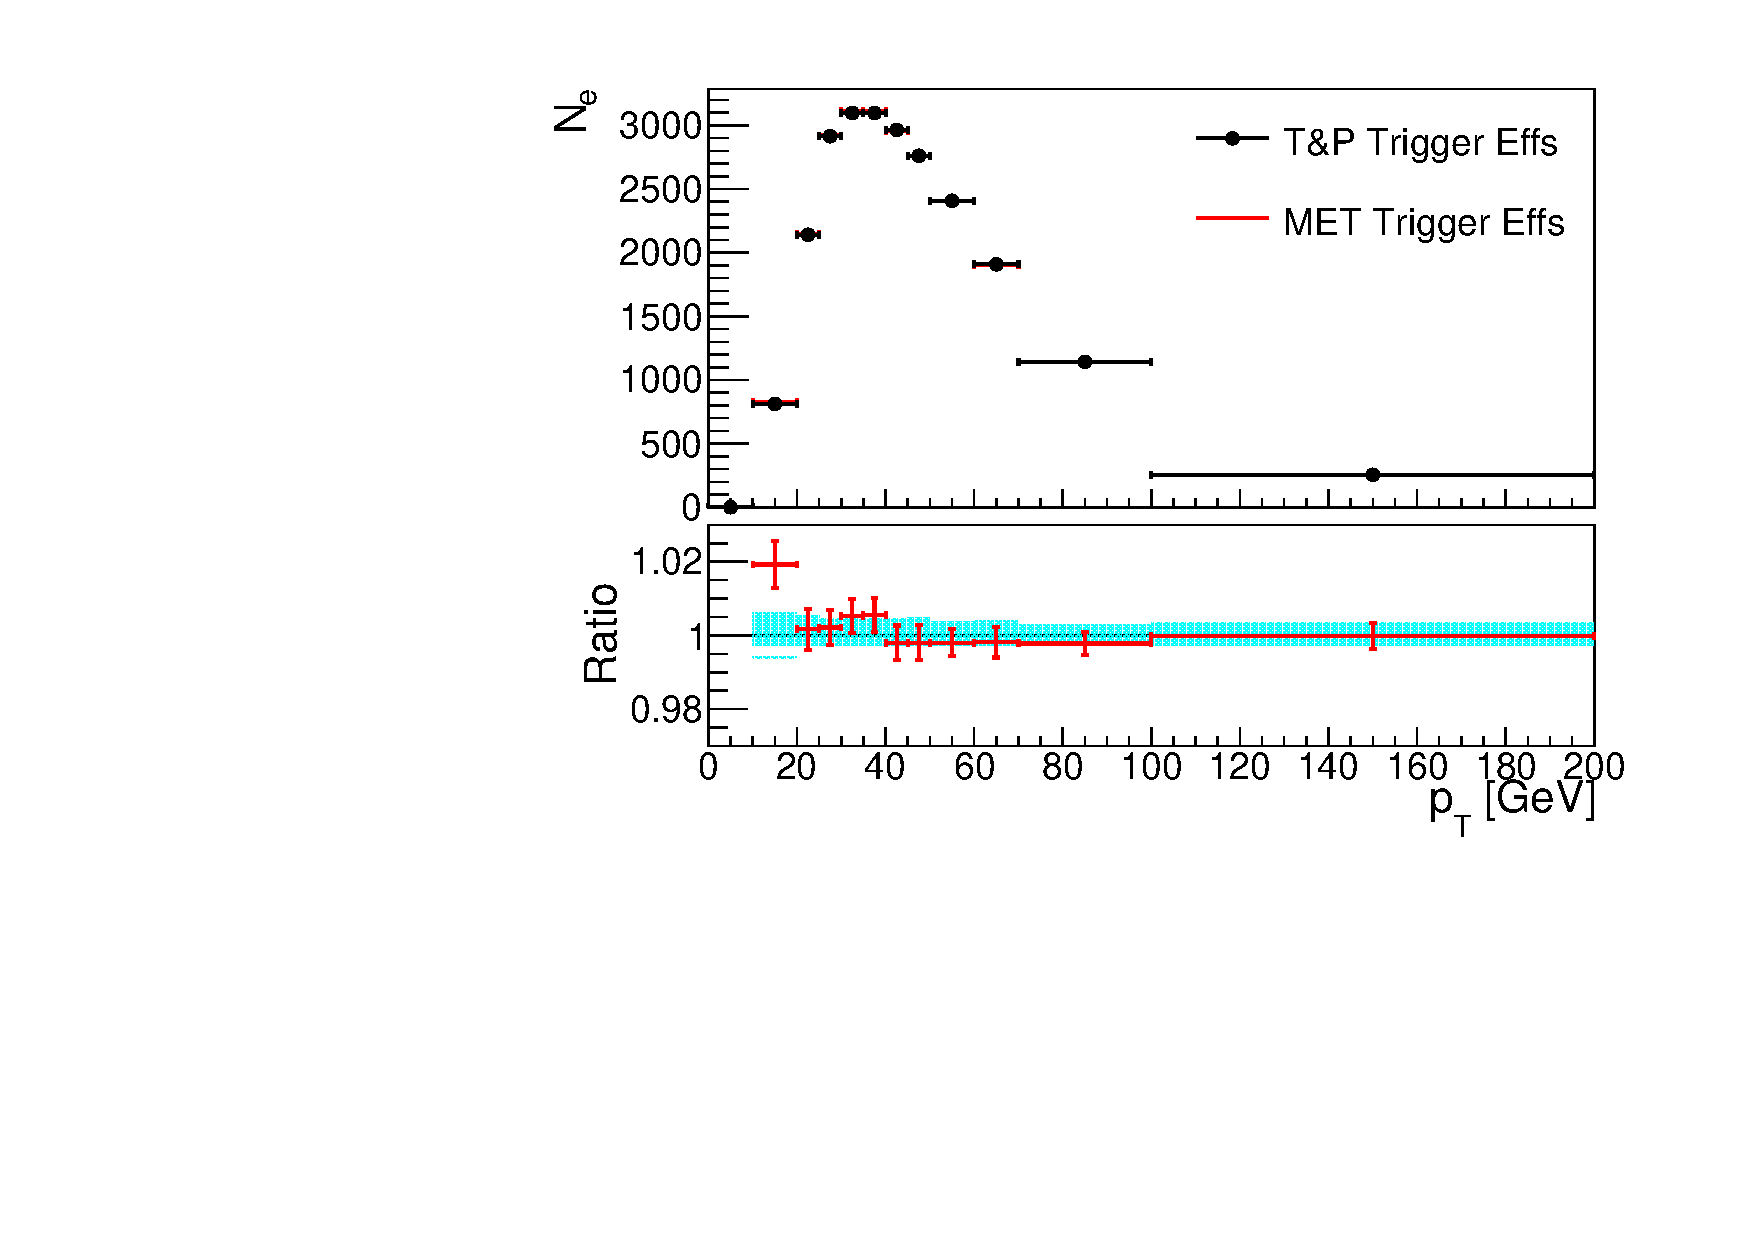
\includegraphics{Trigger/Figures/Clos/emu_ptele}}
    \resizebox{0.48 \textwidth}{!}{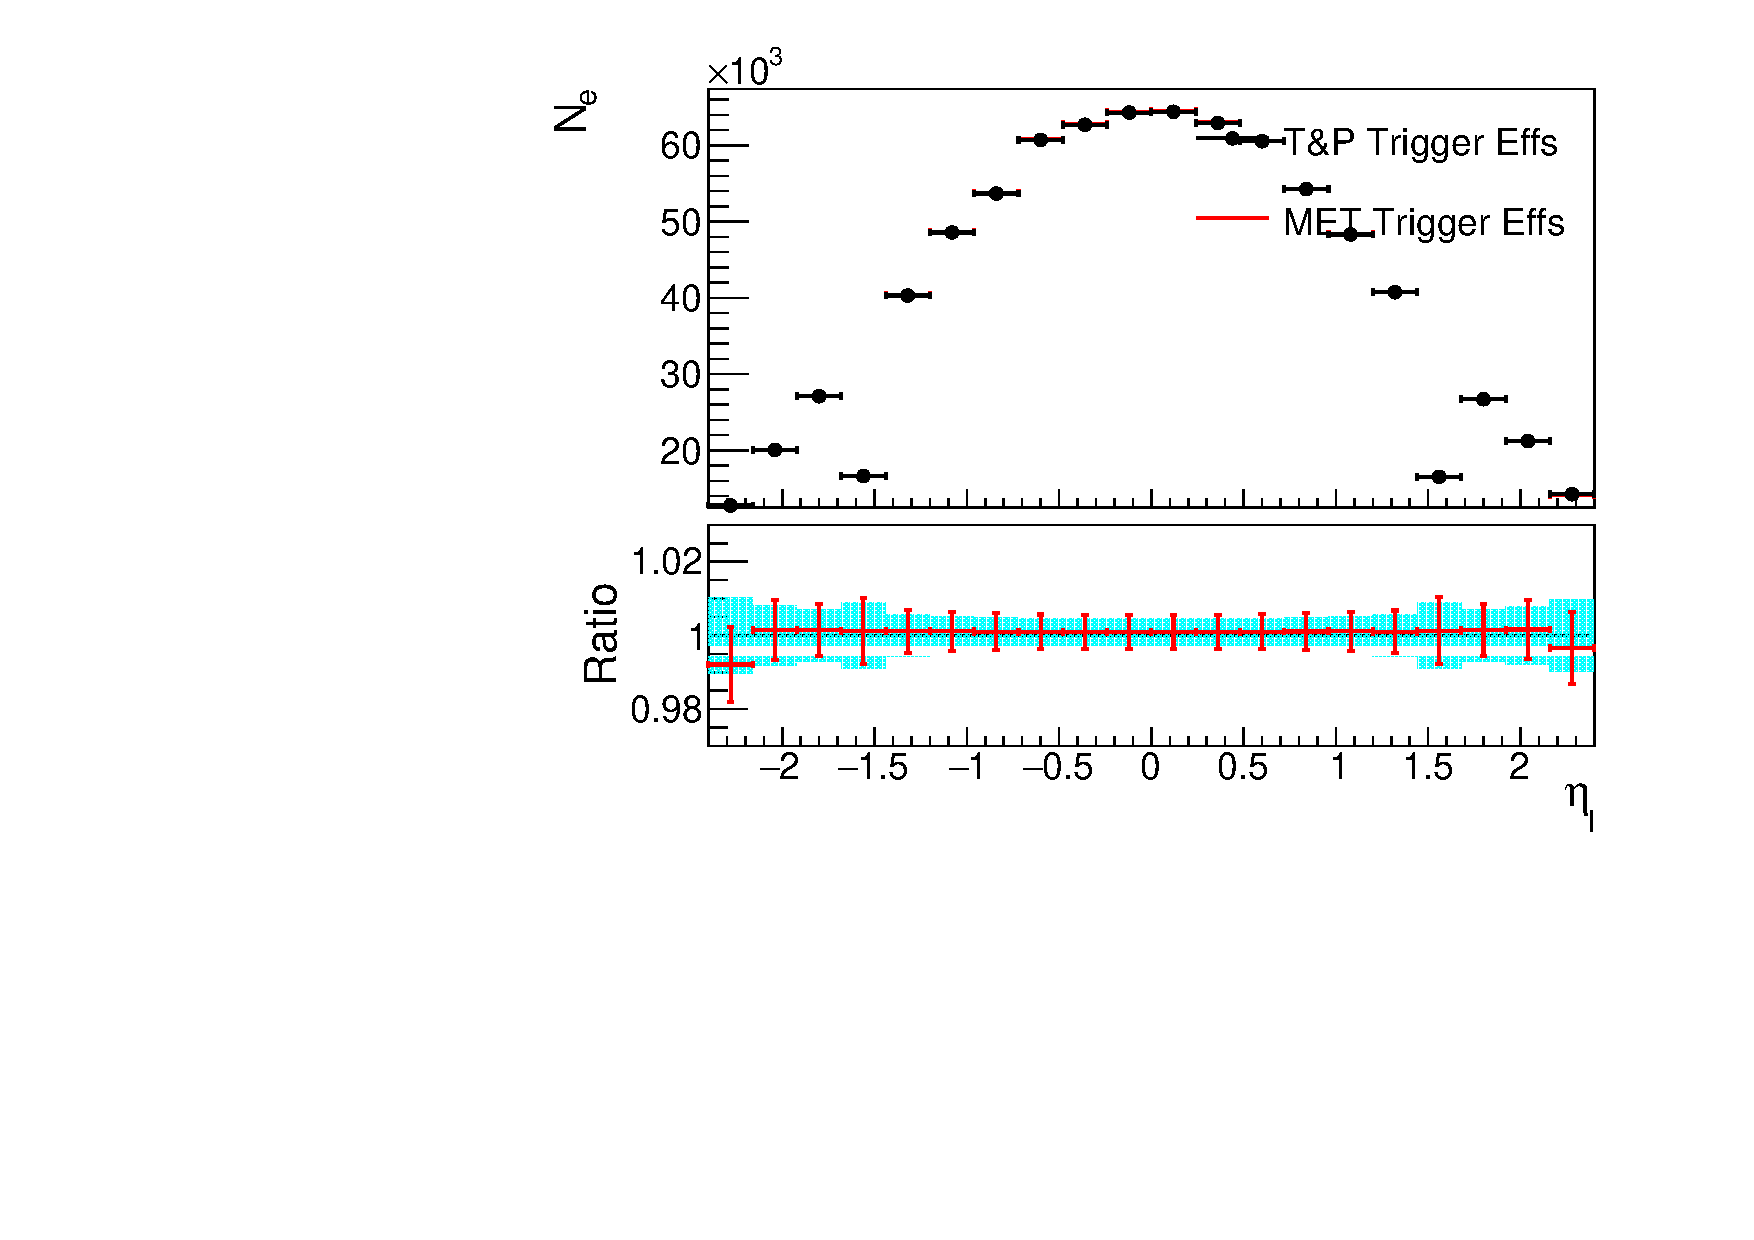
\includegraphics{Trigger/Figures/Clos/emu_etaele}}\\
    \resizebox{0.48 \textwidth}{!}{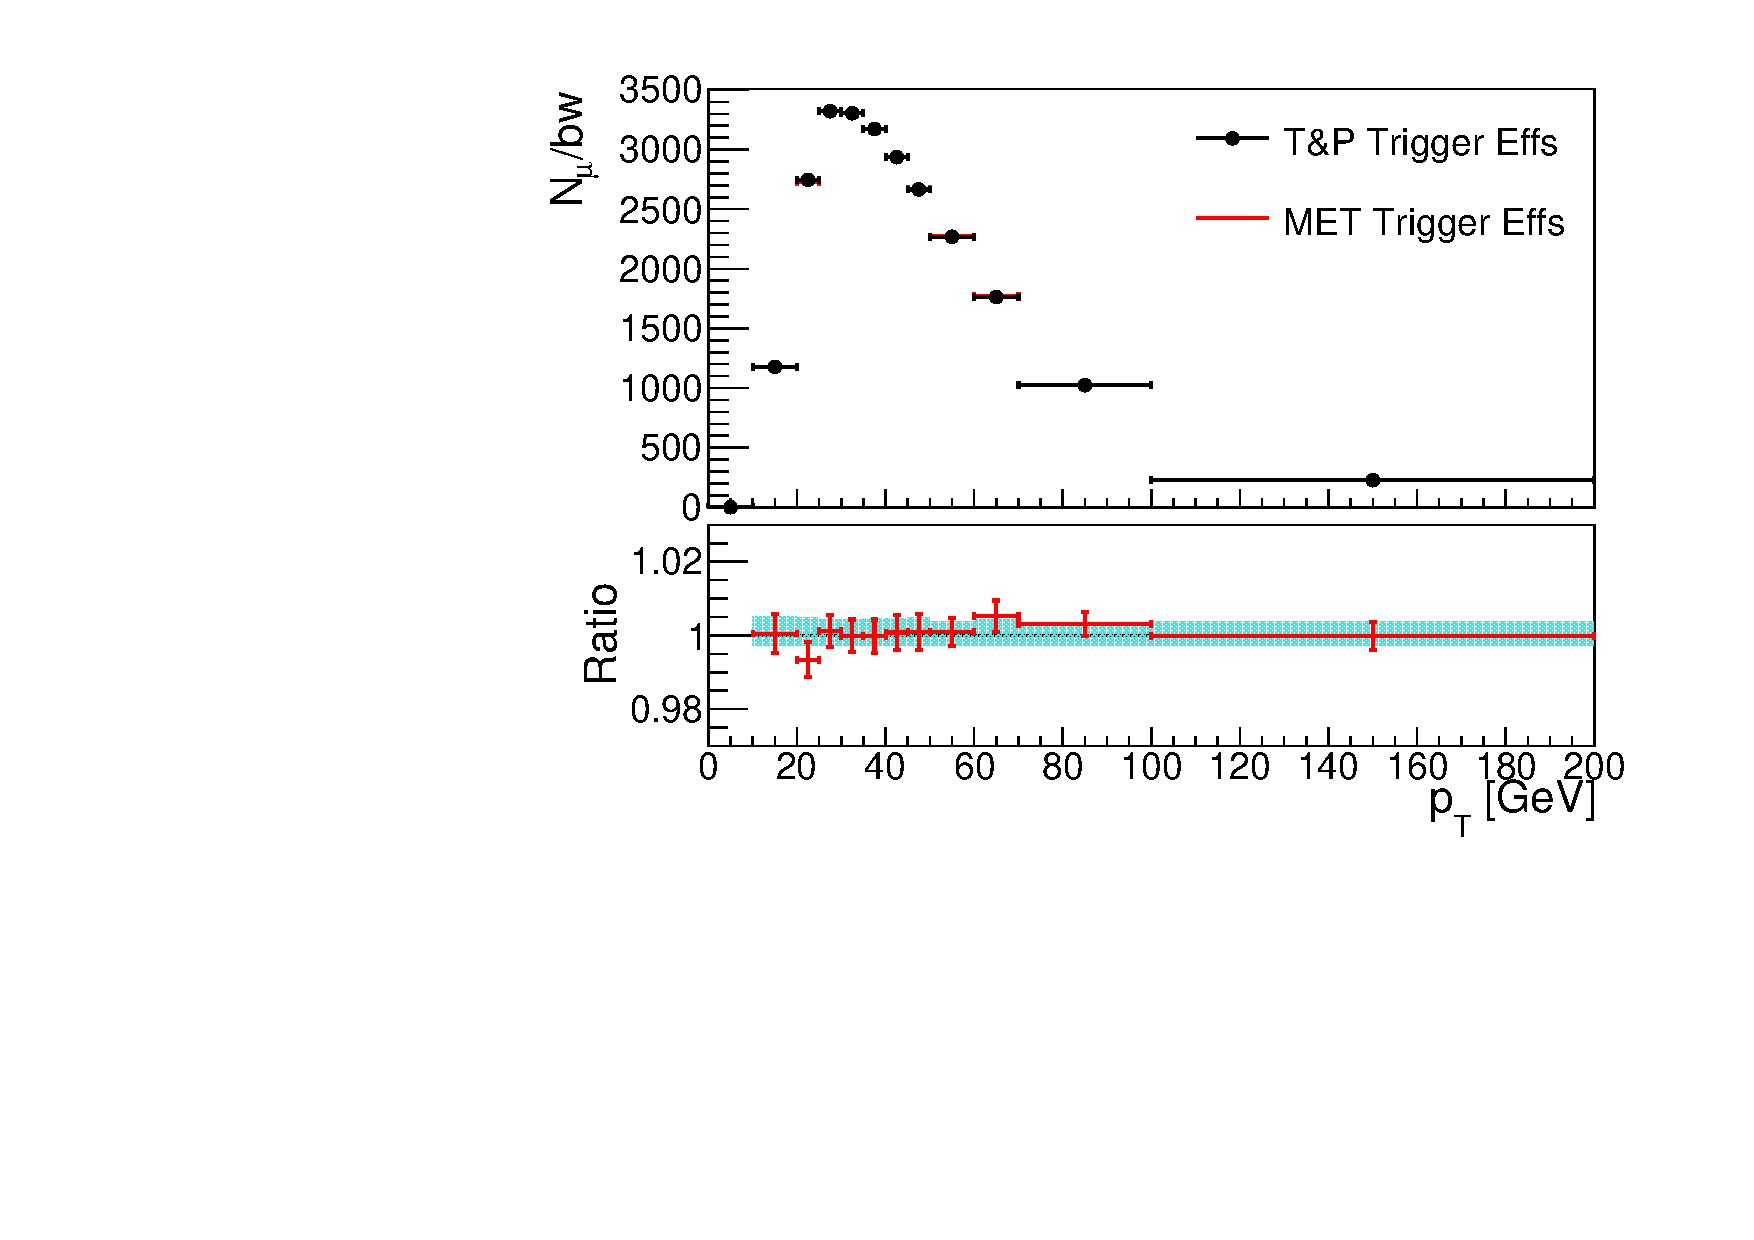
\includegraphics{Trigger/Figures/Clos/emu_ptmu}}
    \resizebox{0.48 \textwidth}{!}{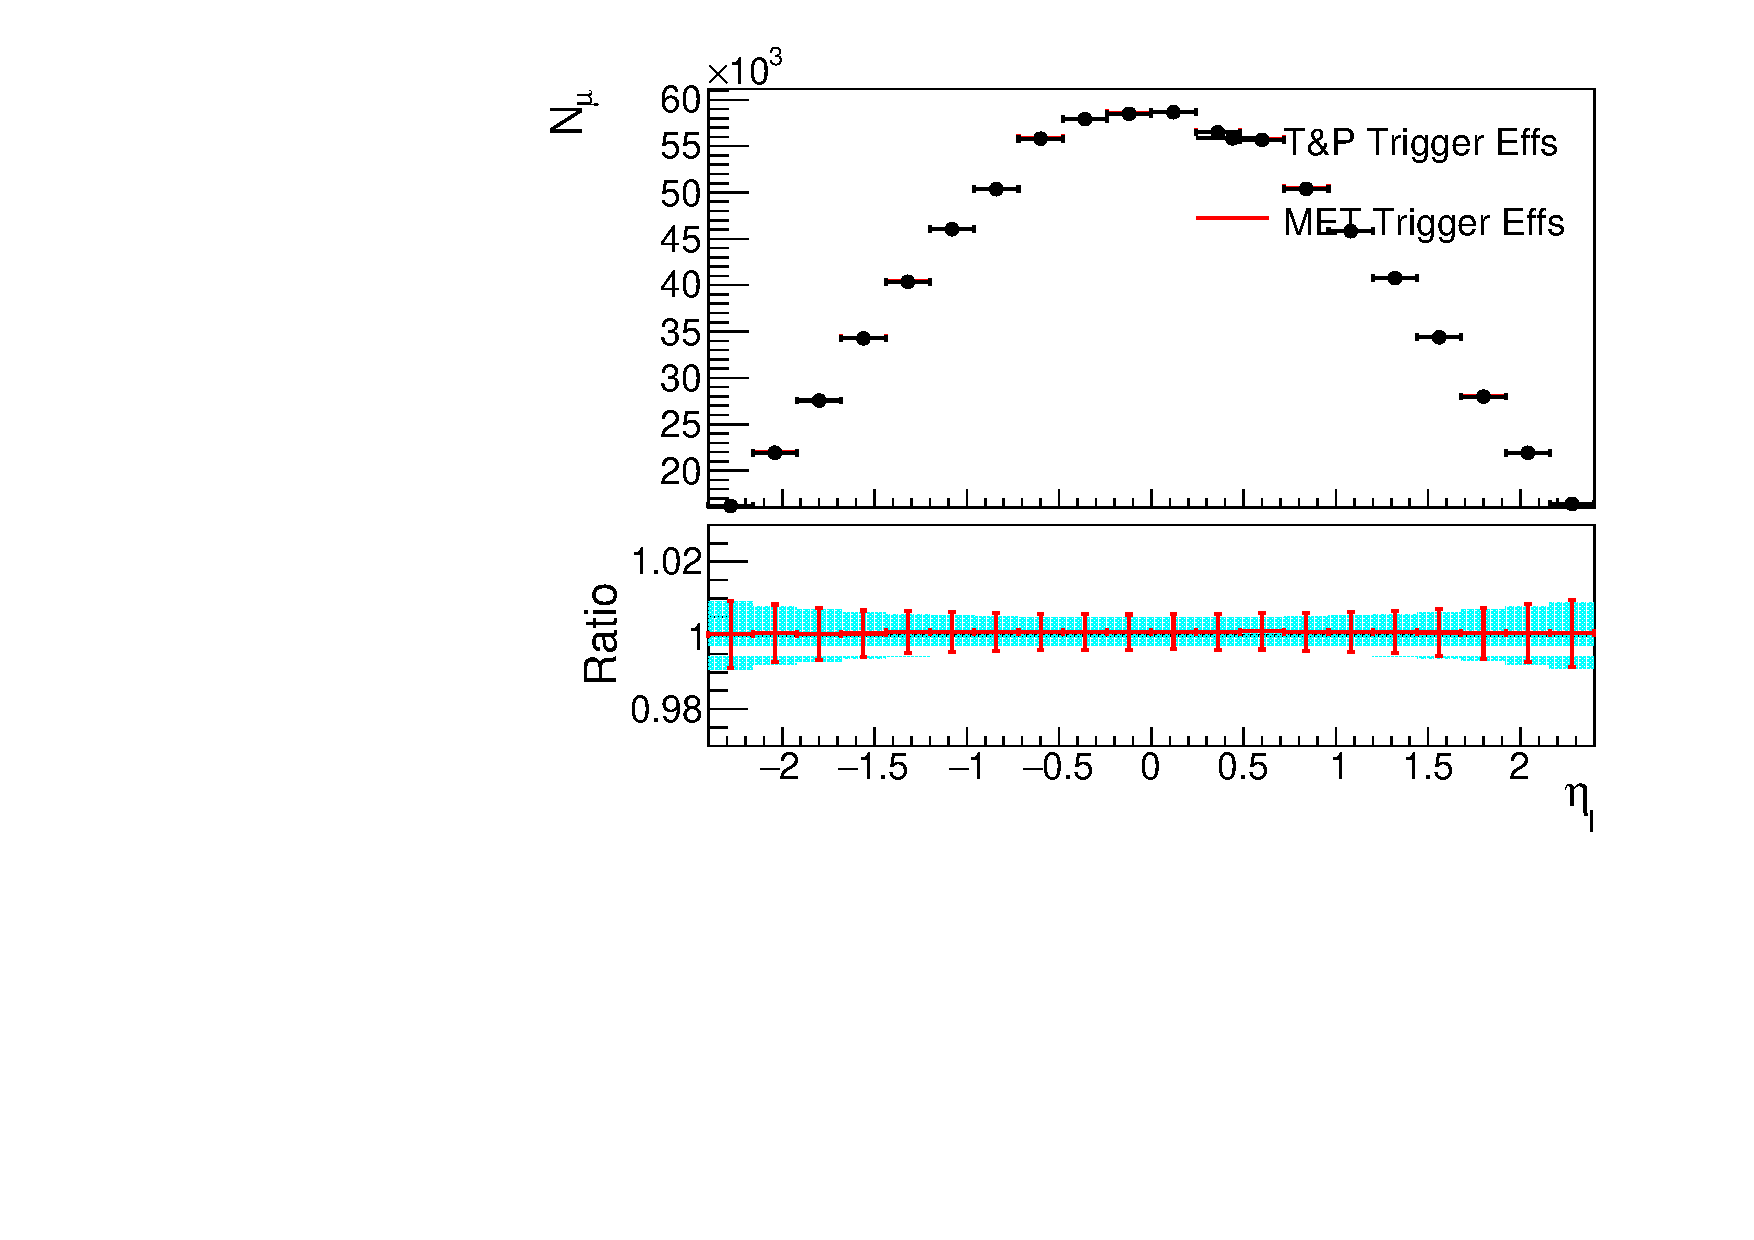
\includegraphics{Trigger/Figures/Clos/emu_etamu}} \\
    \resizebox{0.48 \textwidth}{!}{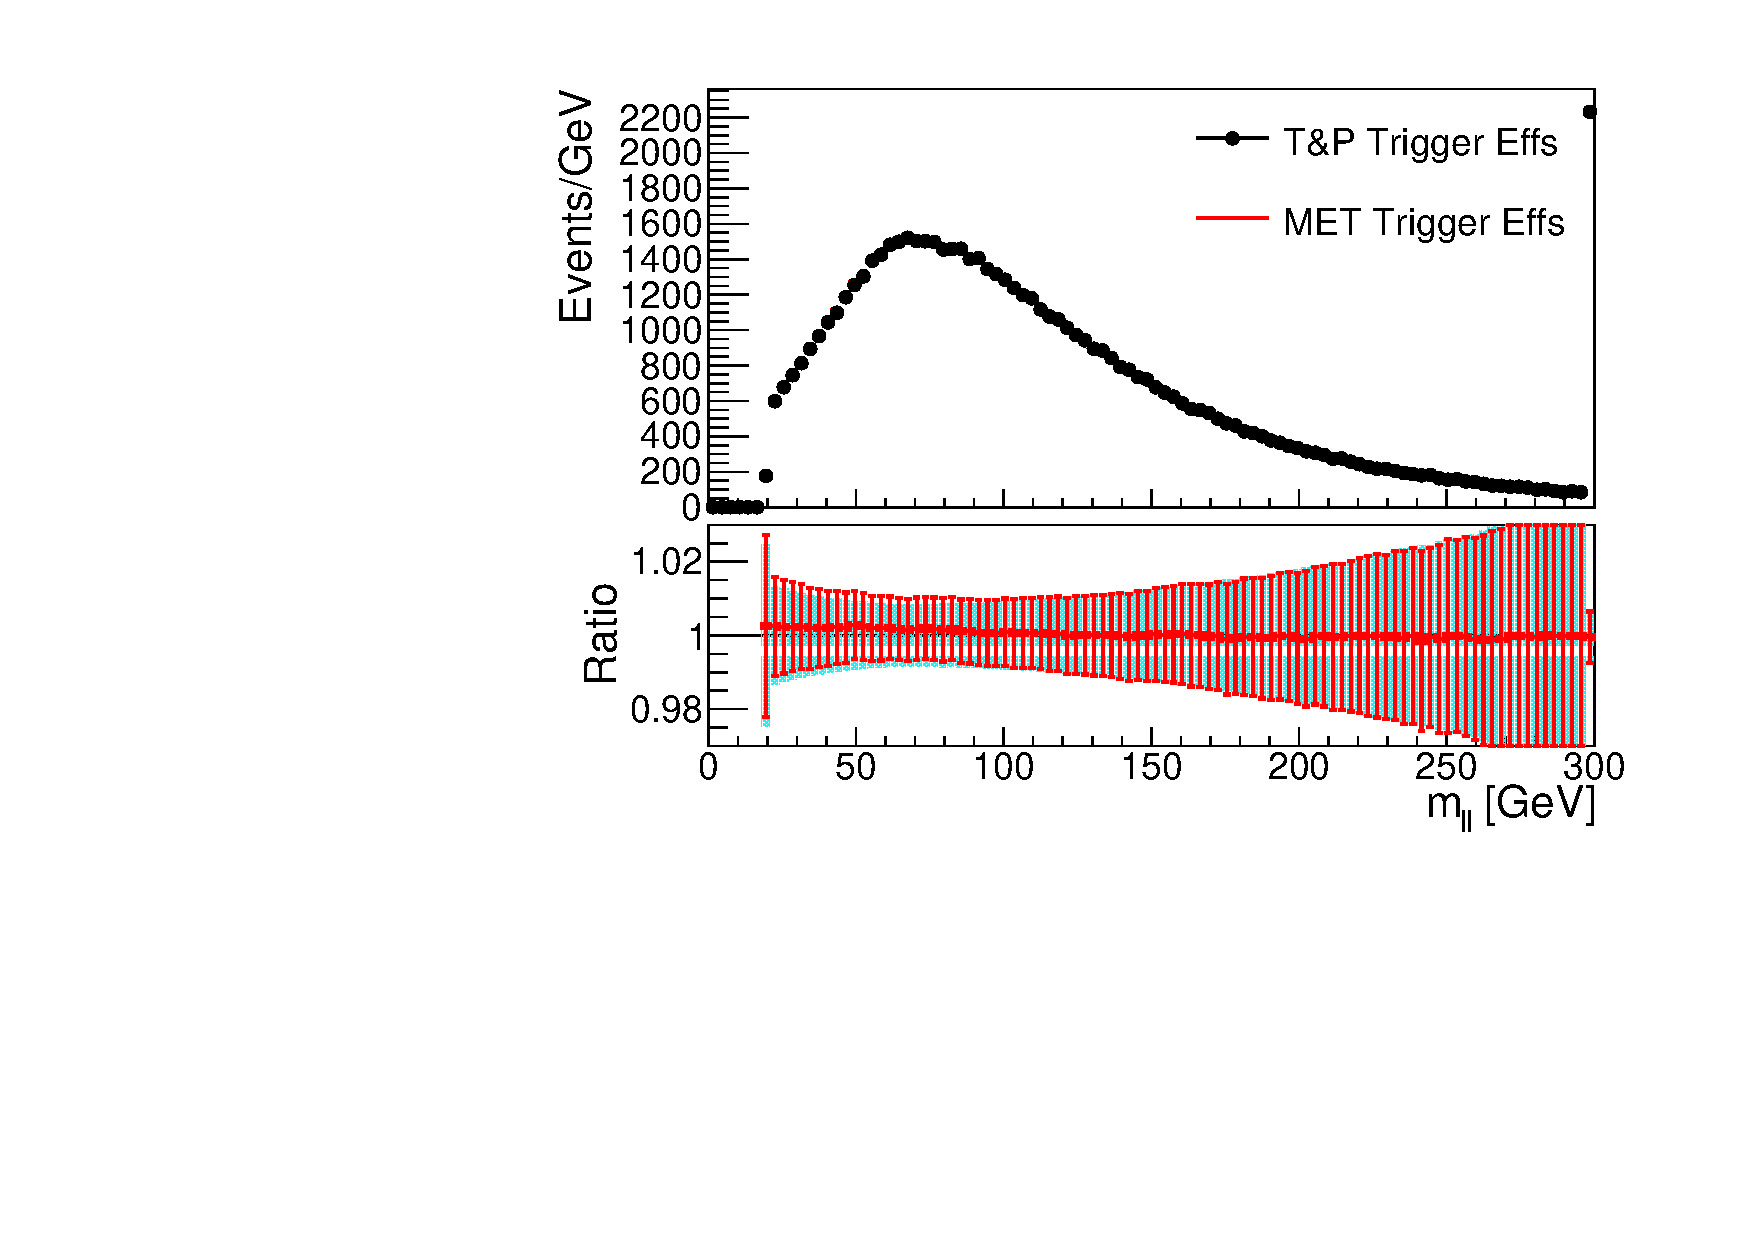
\includegraphics{Trigger/Figures/Clos/emu_mll}}
    \resizebox{0.48 \textwidth}{!}{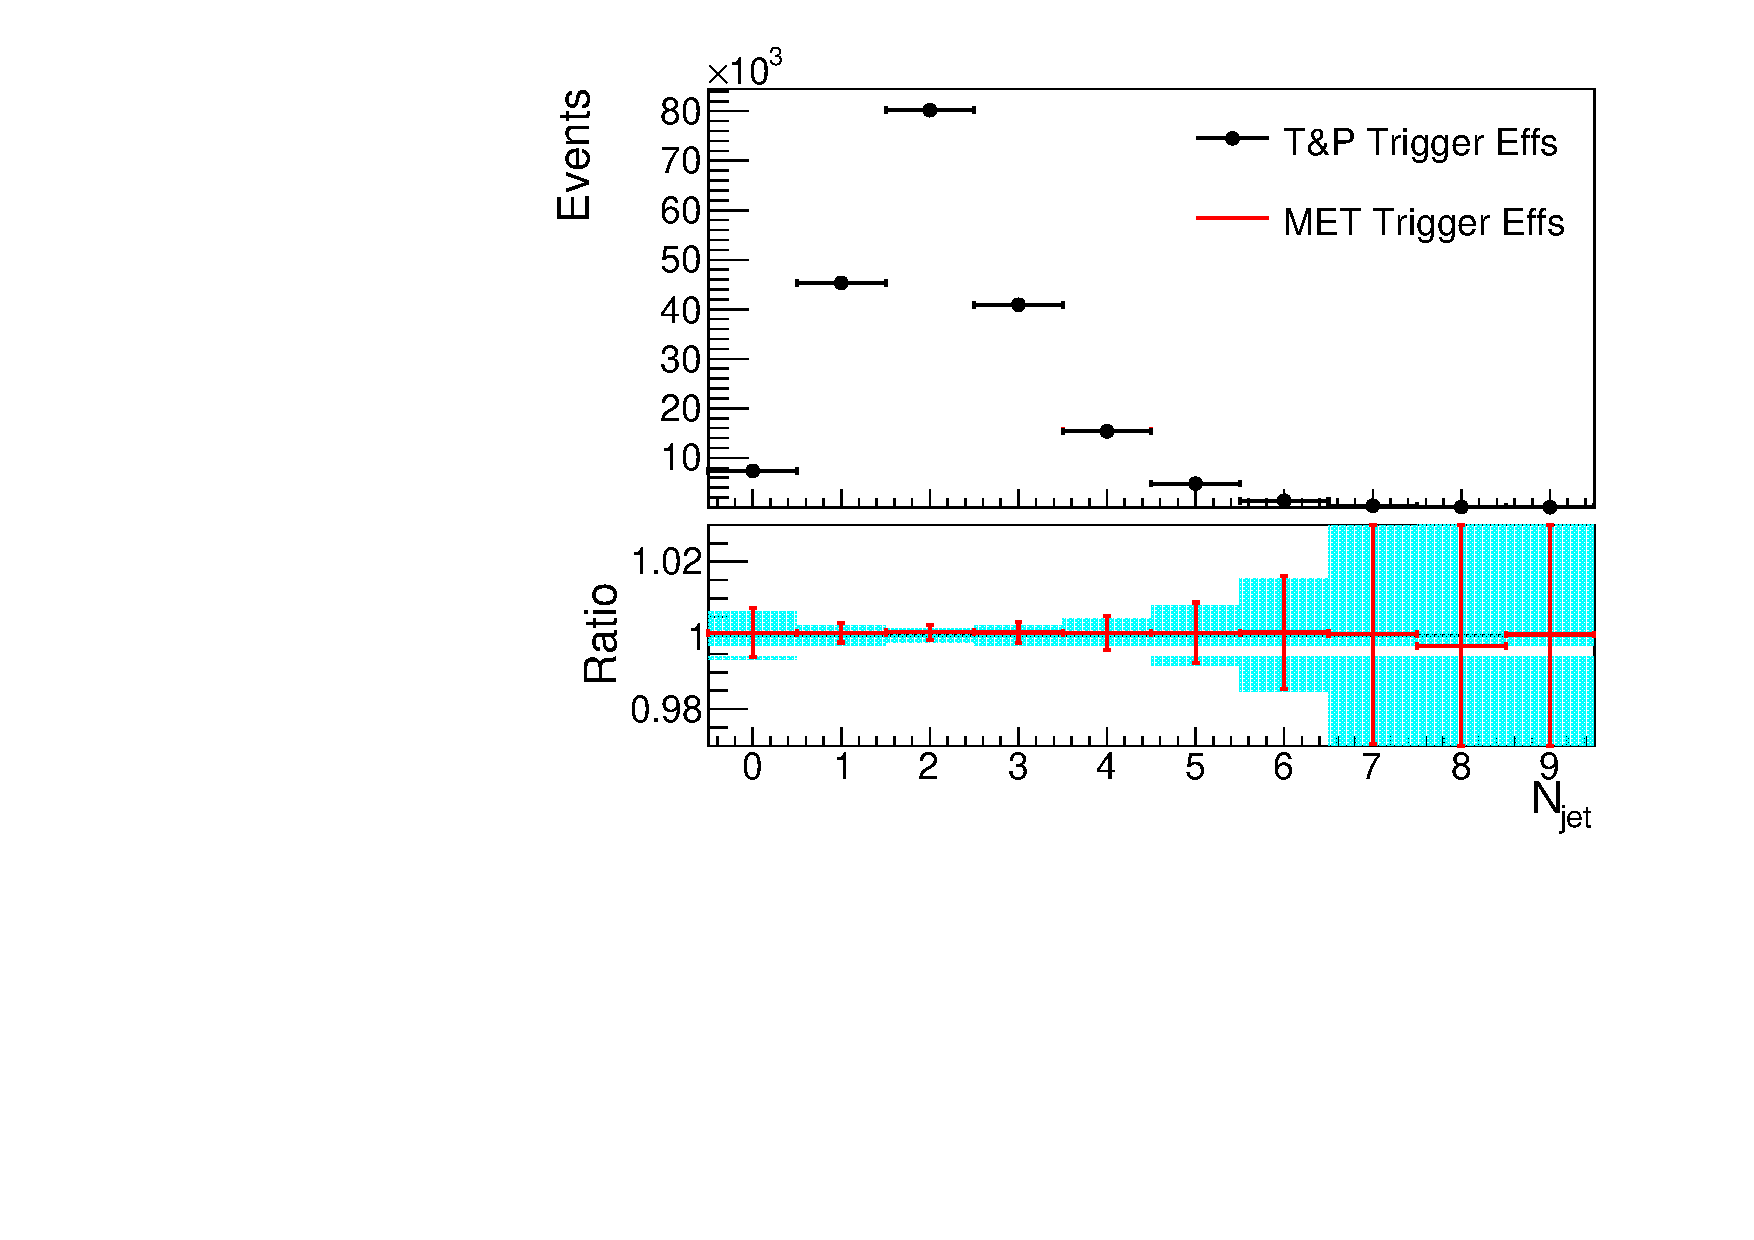
\includegraphics{Trigger/Figures/Clos/emu_njets}}        
      \caption{Comparison of \ttbar simulation reweighted according to the trigger efficiencies measured with the tag-and-probe method and with independent \ETm triggers.
       The upper row shows the comparison in bins of \pt (left) and $\eta$ (right) of the electron. The middle row displays distributions in bins of \pt (left) and $\eta$ (right) of the muon. The lower row displays distributions in bins of the invariant mass of the dilepton system (left) and the number of jets (right). The uncertainties shown are statistical. The lower panels show the ratio of the distribution reweighted with the efficiency from the \ETm trigger method divided by the distribution reweighted by the tag-and-probe method. }  
    \label{fig:Clos_emu}
  \end{center}
\end{figure}

Another way to estimate the systematic uncertainty of the independent trigger method is to compare it to a different set of independent triggers, as described in Section~\ref{sec:TriggerMetMethod}.
Since a set of independent triggers that still delivers enough statistics is hard to find for the dilepton triggers, the trigger efficiency of single-lepton triggers is used for the comparison.
Beside measuring the single-lepton trigger efficiency in a data set triggered by \ETm triggers, it is also measured in a data set triggered by opposite lepton flavor triggers.
So the electron trigger efficiency is measured in a muon data set and the muon trigger efficiency is measured in an electron data set.
The data set triggered by \ETm triggers is dominated by W + jets events, since a lepton and missing transverse energy are required.
The data set triggered with single-lepton triggers is dominated by \ttbar events, as an electron and a muon are required.

The trigger efficiency for each of the single-lepton triggers is measured as a function $\eta$ and \pt in data and simulation for both methods.
Since the phase space for both efficiency measurements is very different, the trigger efficiencies themselves do not necessarily agree with each other.
The scale factor between data and simulation should however agree for both methods.

The comparison is shown in Figure~\ref{fig:Clos_sil} for the single-electron and single-muon trigger efficiency. The efficiency is shown as a function of \pt of the leptons in slices of $\eta$ of the lepton.
The $\eta$ slices are for $|\eta|<0.9$, $|\eta|<1.2$, $|\eta|<2.1$, and $|\eta|<2.4$.
The efficiency for the single-muon trigger is measured in a subset of data, due to problematic conditions for the single-muon trigger in parts of the data.

The scale factors measured for the single-electron trigger with both methods agree in a wide range of the phase space. For $\pt < 20 \GeV$ the two methods do not agree, but that region is not part of the phase space of the analysis.
Similarly, the two methods agree within statistical uncertainties for the full $\eta$ range.

The scale factors measured for the single-muon trigger also agree for most of the phase space. For $\pt > 100 \GeV$ the two methods do not give the same scale factor for two regions of $|\eta|$, but this part of the phase space
is not very relevant for an inclusive \ttbar production cross section measurement.
In summary, no significant systematic difference between the methods is observed.


\begin{figure}[htbp!]
  \begin{center}
    \resizebox{0.75 \textwidth}{!}{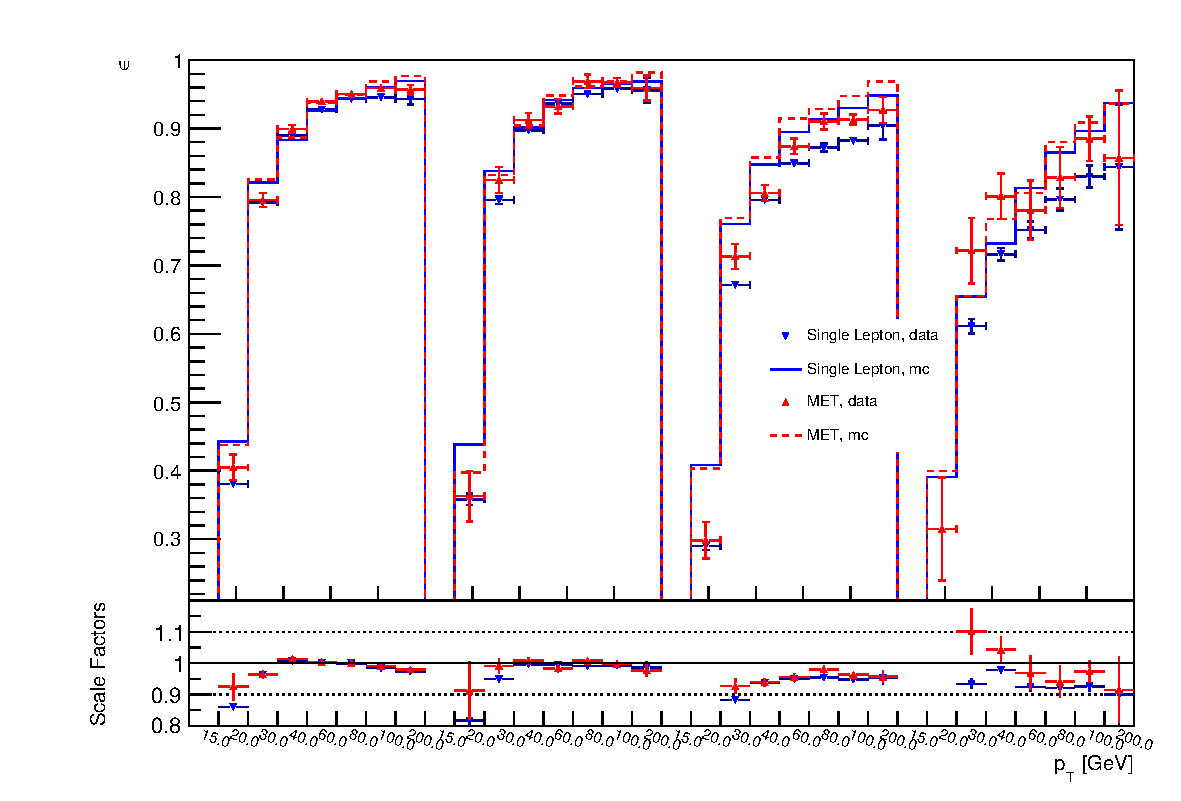
\includegraphics{Trigger/Figures/SingleEle_Comparison}}
    \resizebox{0.75 \textwidth}{!}{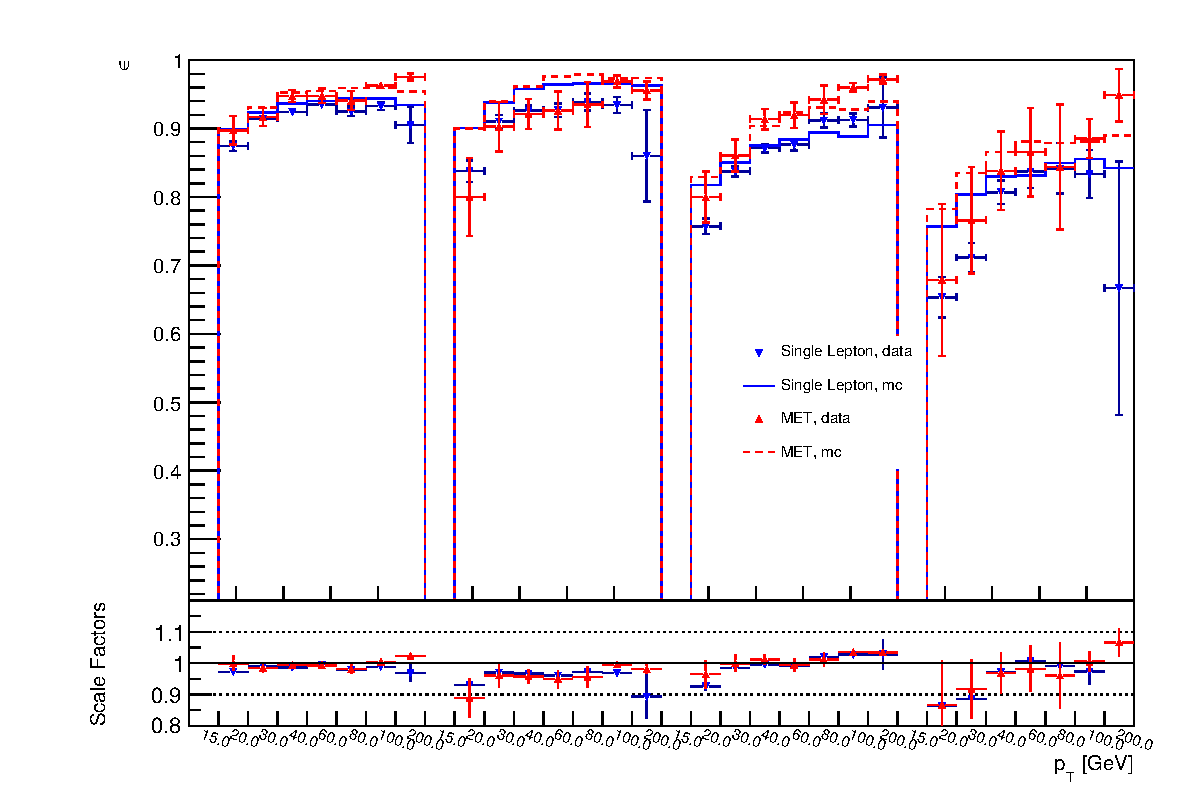
\includegraphics{Trigger/Figures/SingleMu_Comparison_RunG}}        
      \caption{Trigger efficiency for the single-electron trigger (upper figure) and single-muon trigger (lower figure) as a function of \pt in slices of $\eta$. The efficiency is measured in data and simulation with the independent trigger method. For the single-electron trigger the independent triggers are either single-muon triggers or \ETm triggers. For the single-muon trigger the independent triggers are either single-electron triggers or \ETm triggers.
      The lower panels show the scale factor between data and simulation for both methods. The uncertainties shown are statistical uncertainties.}  
    \label{fig:Clos_sil}
  \end{center}
\end{figure}



\section{Determination of the trigger scale factor}

\label{sec:TrigSF}

The scale factors that correct the trigger efficiency in simulation to the data are determined using the independent trigger method with \ETm triggers, as described in Section~\ref{sec:TriggerMetMethod}. 
It has advantages over the tag-and-probe method: it measures the trigger efficiency directly per event for the complete trigger selection and does not require any additional assumptions on the correlations between the triggers.

Based on the comparison of the two methods (see Section~\ref{sec:TriggerComp}) and the additional study of the single-lepton triggers, a remaining systematic uncertainty of $0.3\%$ is applied in addition to the statistical uncertainty.
Systematic and statistical uncertainty are added in quadrature. 

The scale factors are binned in $|\eta|$ of the two leptons, as shown in Figure~\ref{fig:TrigSF}. This provides a good compromise between covering disagreements between data and simulation seen in Section~\ref{sec:TriggerMetMethod} and sufficient statistical power for each bin.


\begin{figure}[htbp!]
  \begin{center}
    \resizebox{0.48 \textwidth}{!}{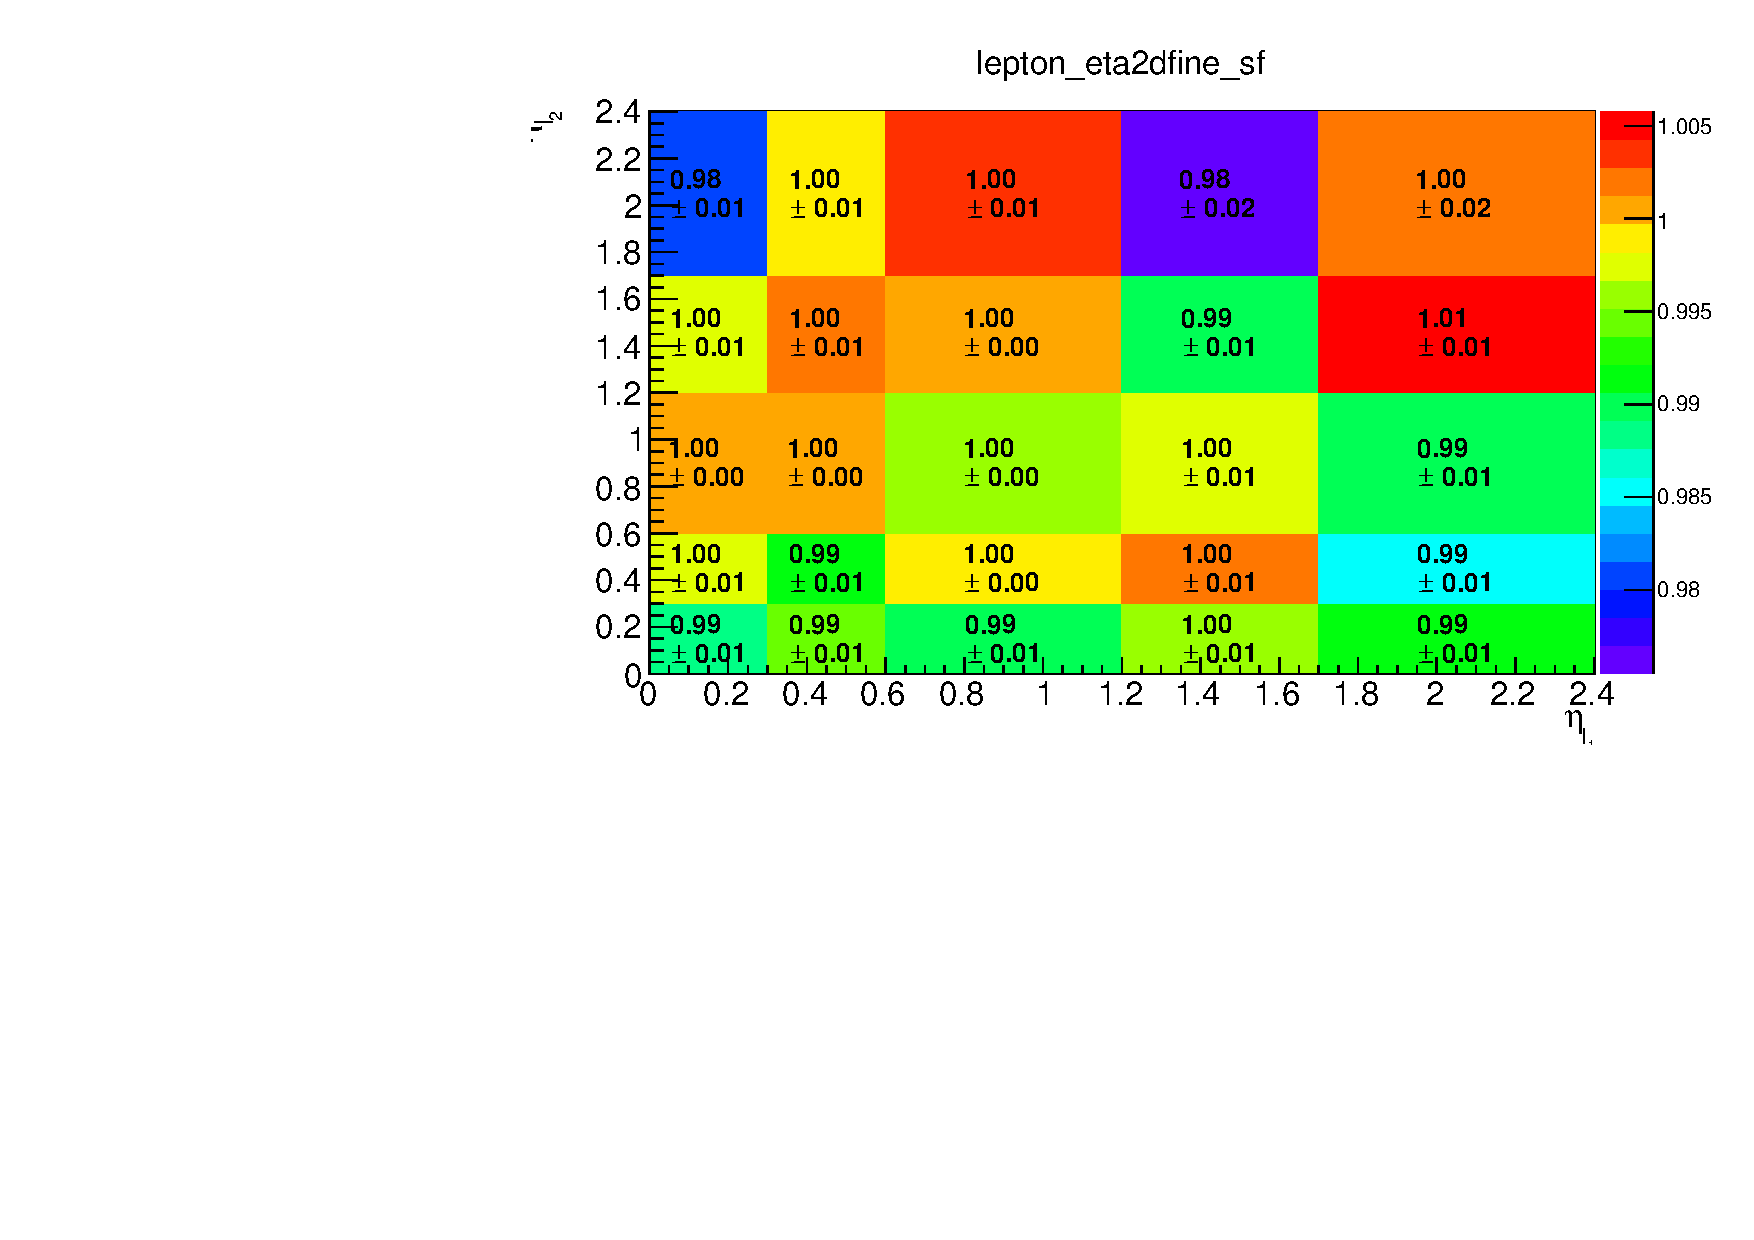
\includegraphics{Trigger/Figures/emu_eta2d_sf}}
    \resizebox{0.48 \textwidth}{!}{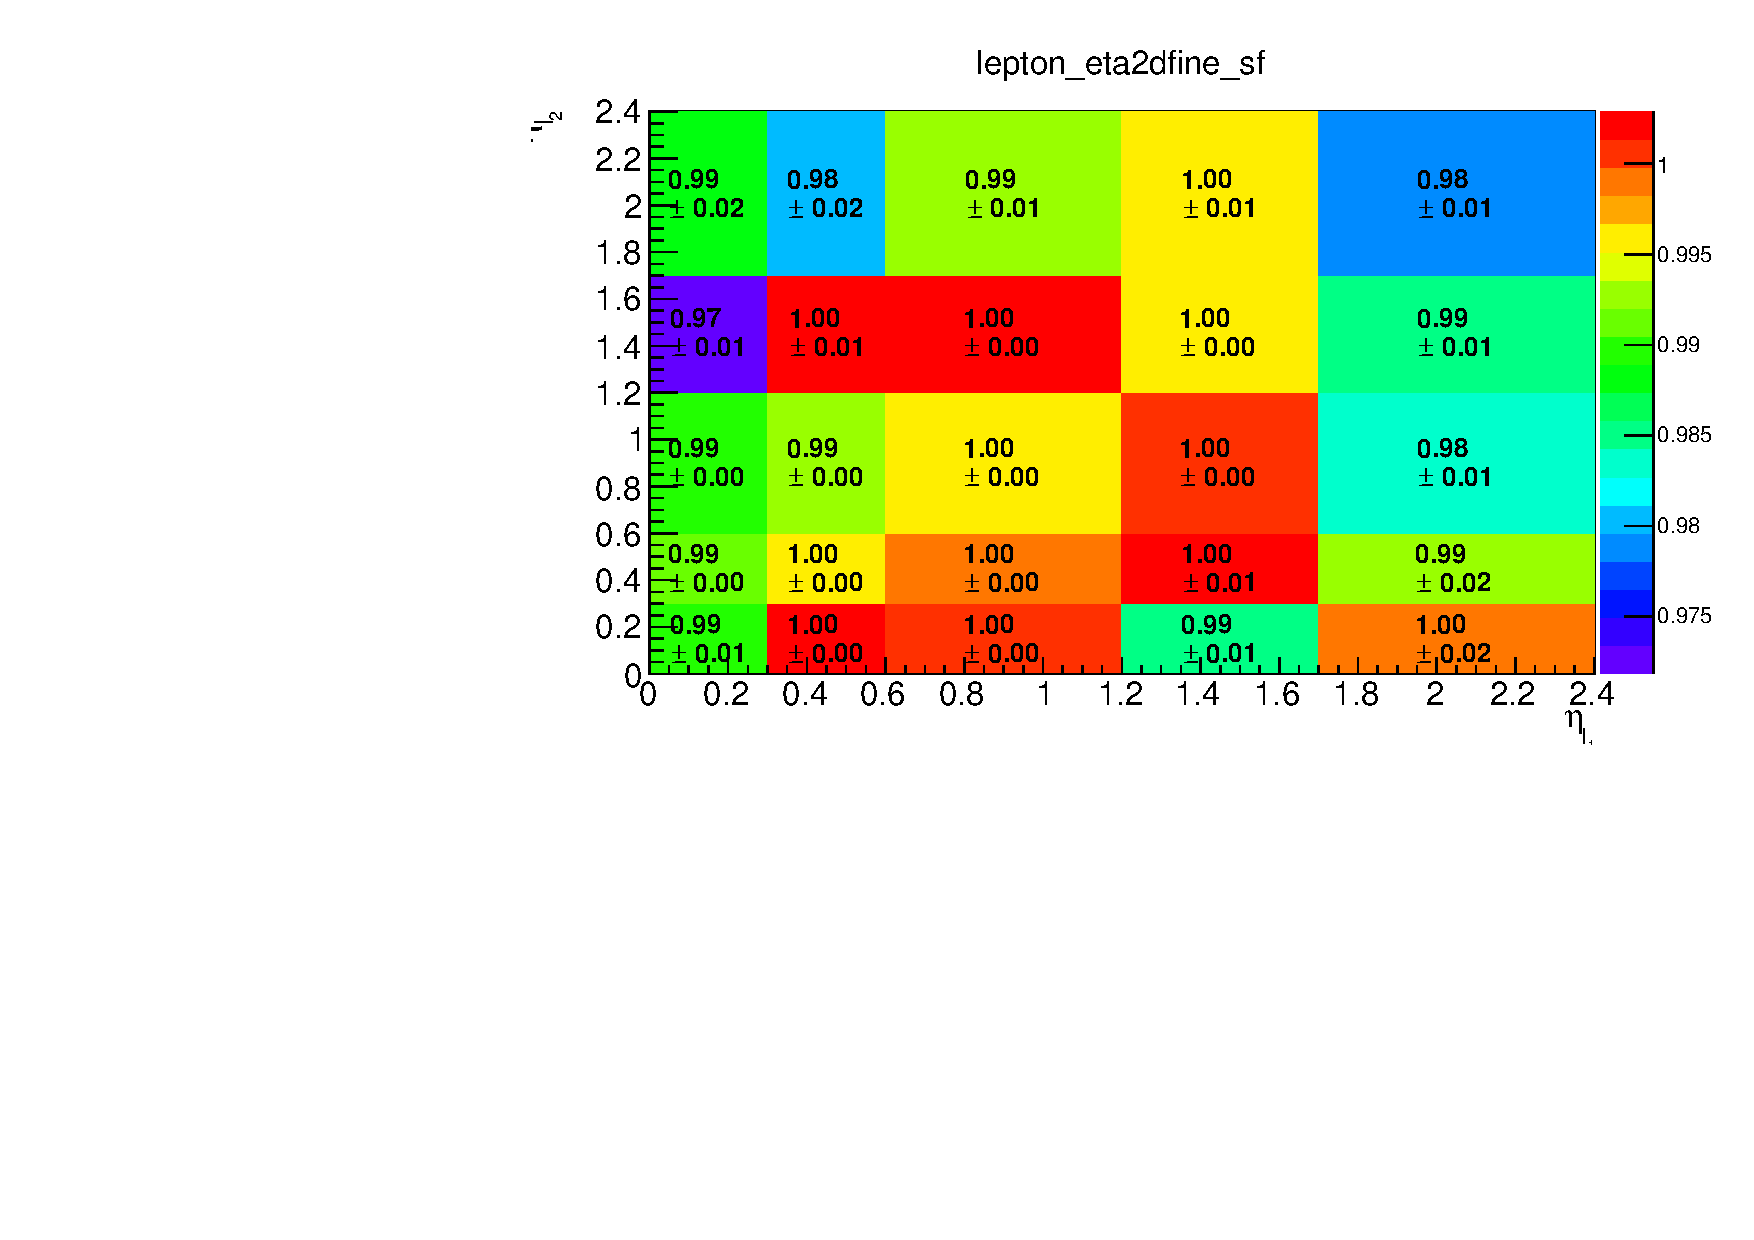
\includegraphics{Trigger/Figures/mumu_eta2d_sf}}\\
    \resizebox{0.48 \textwidth}{!}{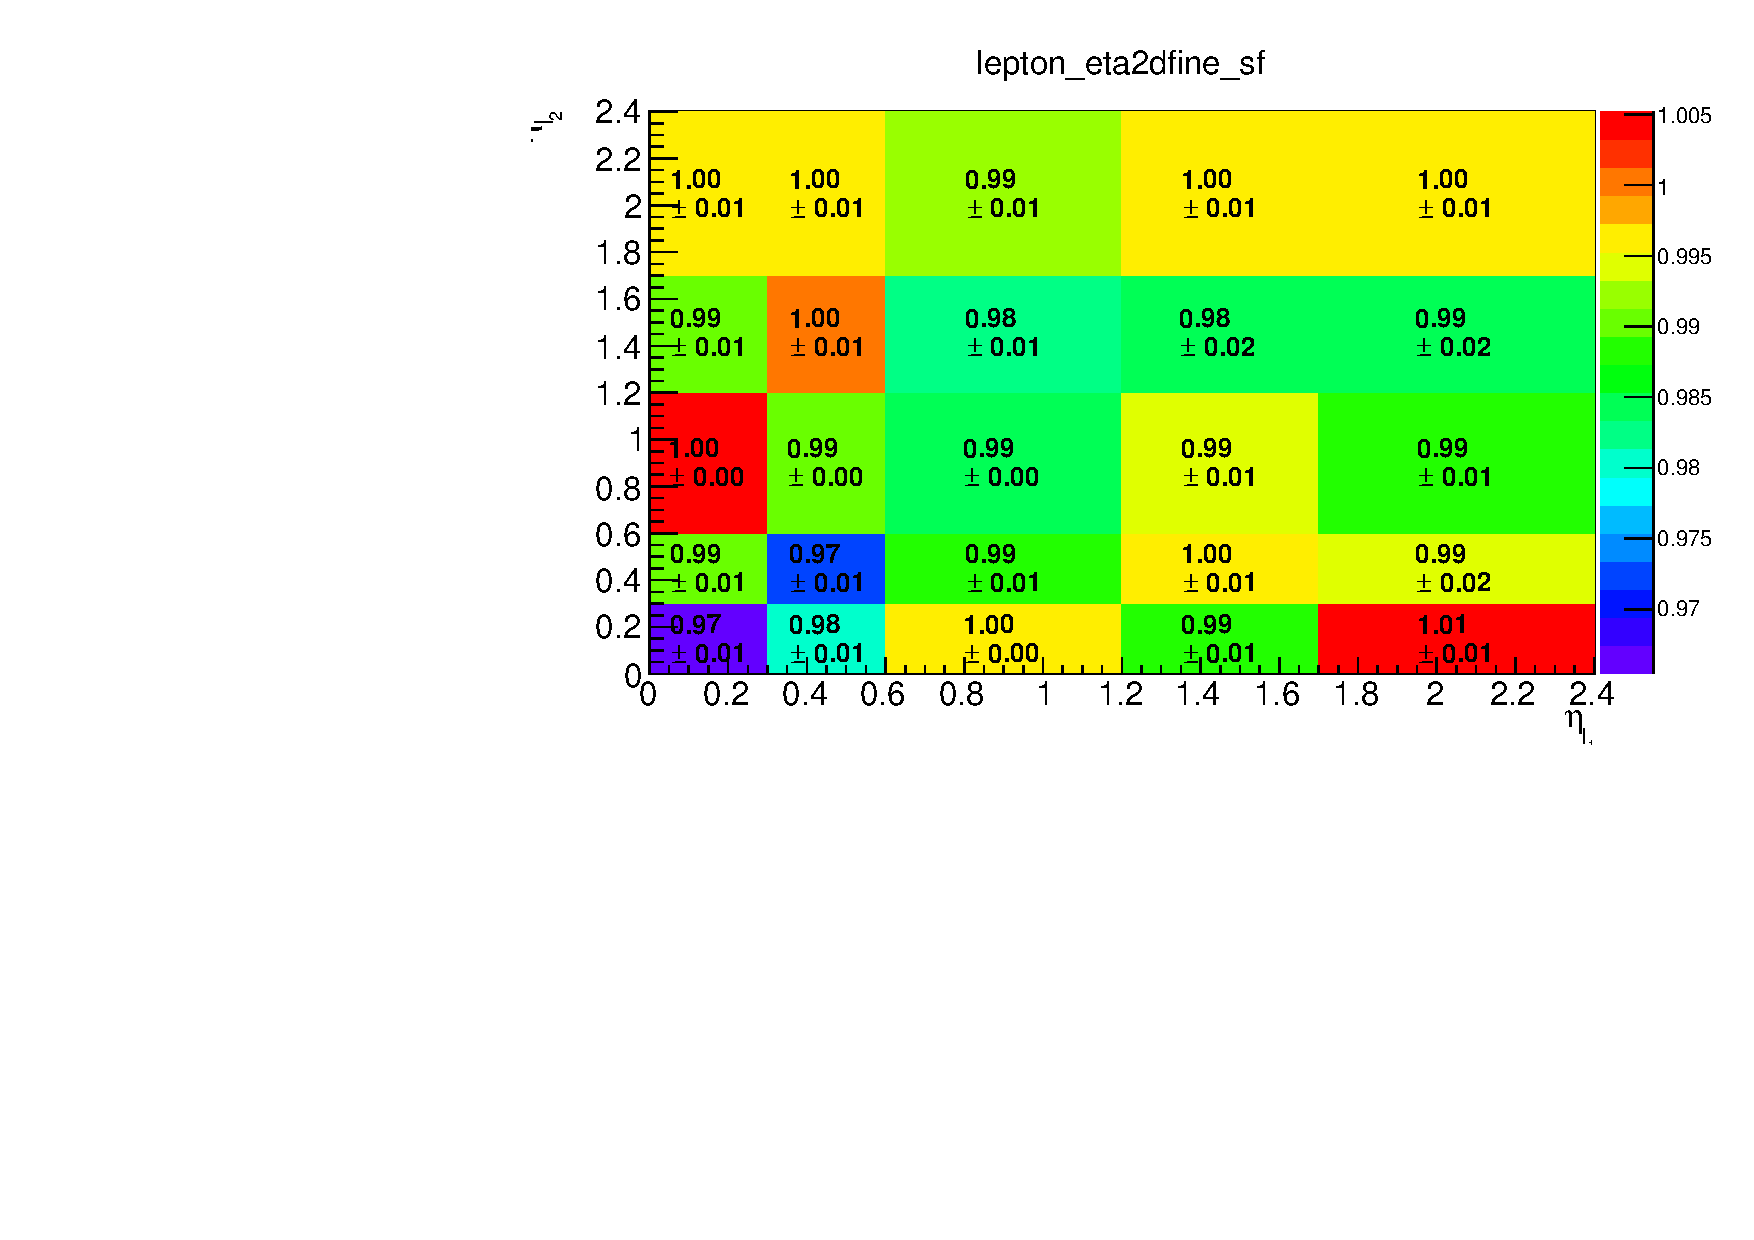
\includegraphics{Trigger/Figures/ee_eta2d_sf}}       
      \caption{Scale factors from the trigger efficiencies of the trigger selection in the \emu (upper left), \mumu (upper right) and \ee (lower middle) channel. The scale factors are given in bins of the $|\eta|$ of the two leptons. The uncertainties denote the combination of statistical and systematic uncertainties.}  
    \label{fig:TrigSF}
  \end{center}
\end{figure}

With the trigger efficiency determination all necessary corrections to simulation are made and the \ttbar cross section can be measured. This measurement is described in the following chapter.






